\documentclass{jvfscript-de}
\usepackage{diff3style}
\usepackage{graphicx}
\graphicspath{ {./images/} }

%\usepackage{showframe}

\makeindex[title=Definitionen,intoc]

\renewcommand{\thechapter}{\S \arabic{chapter}}
\renewcommand{\thesection}{\arabic{chapter}.\arabic{section}}
\renewcommand{\thethm}{\arabic{chapter}.\arabic{thm}}
 
%\includeonly{./lectures/cpt07 }

\hypersetup{
	colorlinks=true,
	linkcolor=blue,
	filecolor=blue,      
	urlcolor=blue,
	pdftitle={Vorlesungsskript Diff 3},
	bookmarks=true,
%	pdfpagemode=FullScreen,
	bookmarksopen = true
}

\begin{document}
	\frontmatter
	\maketitle
	
%	\setcounter{page}{1}
\tableofcontents
\newpage
%	\setcounter{page}{1}
\thispagestyle{plain}
Dieses Skript stellt keinen Ersatz für die Vorlesungsnotizen von Prof. Bahns dar und wird nicht nochmals von ihr durchgesehen, im Grunde sind das hier nur meine persönlichen Mitschriften. Beweise werde ich i.d.R. nicht übernehmen (weil das in \LaTeX{} einfach keinen Spaß macht). \hspace{\fill} glhf
\newpage
\mainmatter
\setstretch{1.15}			%Zeilenabstand. Kann man auch später nochmal reinhämmern, falls man es ändern will
	
	
	
	
	
	\chapter{Mannigfaltigkeiten}\lecture

\begin{defn}[Topologische Mannigfaltigkeit]\label{def1_1}\index{Mannigfaltigkeit}
	Eine \emph{$n$-dimensionale topologische Mannigfaltigkeit $M$} ist ein topologischer Hausdorff-Raum mit abzählbarer Basis der Topologie, der lokal euklidisch ist.
	\begin{itemize}
		\item lokal euklidisch:\\
			$ \foralll p \in M\ \existss U $ offene Umgebung von $p$, die homöomorph zu einer offenen Teilmenge des $\R^n$ ist, das heißt es gibt eine stetige, injektive Abbildung $ \varphi: U \to \R^n $ mit $ \varphi(U) $ offen in $\R^n$ (mit der Standardtopologie) und mit stetiger Umkehrfunktion $\varphi^{-1}: \varphi(U) \to M$.
			\image{1_1 homoeo}{12cm}
			\begin{rem*}
				$\varphi$ und auch $\varphi^{-1}$ sind offene Abbildungen, denn Bilder offener Mengen $ \tilde{U} \subset U $ (bezüglich $\varphi$), also $ \varphi(\tilde{U}) \subset \varphi(U) = \im(\varphi) $, sind Urbilder (bezüglich $\varphi^{-1}$) offener Mengen $\tilde{U}$ und somit offen (wegen der Stetigkeit von $\varphi^{-1}$)
				\image{1_1 offen}{8cm}
				Das heißt $U$ und $\varphi(U)$ sind als topologische Räume äquivalent (weil ihre offenen Mengen in $1-1$-Beziehung zueinander stehen).
			\end{rem*}
		\item Hausdorff-Raum:\\
			$ \foralll p \neq q \in M \ \existss U,V \subset M $ offen, sodass $ U \cap V = \emptyset,\ p \in U, q \in V $
			\image{1_1 hausdorff}{6cm}
			Erinnerung: In topologischen Räumen mit Hausdorff-Eigenschaft sind z.B. Grenzwerte von konvergenten Folgen eindeutig.
		\item Abzählbare Basis der Topologie:\\
			Es gibt ein höchstens abzählbares System $ \{U_1,U_2,U_3,\dots\} $ von offenen Mengen $ U_j \subset M $, sodass $ \foralll p \in M \ \forall $ Umgebungen $V$ von $p$ gibt es einen Index $j$, sodass $ p \in U_j \subset V $.
			\begin{rem*}
				Warum man dies fordert werden wir später bei der Existenz einer Teilung der Eins erkennen.
			\end{rem*}
	\end{itemize}
	\begin{notat*}
		Ist $M$ eine topologische Mannigfaltigkeit, $p \in M$, so nennt man einen Homöomorphismus $\varphi: U \to \tilde{U}$, $U$ offen in $M$, $\tilde{U} = \varphi(U)$ offen in $\R^n$, $p \in U$, eine \emph{(lokale) Karte} bei $p$. Gilt $ \varphi(p) = 0 $, sagt man, die Karte sei zentriert bei $p$.\\
		$U$ heißt \emph{Koordinatenbereich} von $\varphi$ und die Komponenten von $\varphi(q) = (x_1(q),\dots,x_n(q))$ (für $q \in U$) heißen \emph{lokale Koordinaten} von $q$.
		\begin{rem*}
			Ist $\varphi$ eine beliebige Karte bei $p$, so ist $\psi(q) = \varphi(q) - \varphi(p)$ eine bei $p$ zentrierte Karte.
		\end{rem*}
	\end{notat*}
	Ein System von Karten $ \set{(\varphi_\alpha,U_\alpha)}{\alpha \in A} $ heißt \emph{Atlas} von $M$, falls gilt $ M = \bigcup\limits_{\alpha \in A} U_\alpha $.
\end{defn}

\begin{exmp}
	\begin{enumerate}[label= {\roman*})]
		\item $M = \R^n$, versehen mit der Standardtopologie, denn $ \varphi: \R^n \to \R^n,\ \varphi(x) = x $ ist ein Homöomorphismus. $\R^n$ ist ein Hausdorff-Raum (vlg. Diff 2) und verfügt über eine abzählbare Basis: $ \set{\dot{B_r}(q) \ \text{offener Ball}}{r \in \Q, p \in \Q^n}. $
		\item Graphen von stetigen Funktionen:\\
			$ U \subset \R^n $ offen, $f: U \to \R^k$ stetig. Der \emph{Graph} $ \Gamma(f) = \set{(x,f(x))}{x \in U} \subset \R^n \times \R^k $, versehen mit der \emph{Teilraumtopologie}\footnote{
				Eine Teilmenge $M\subset \R^m$ ist mit der Teilraumtopologie versehen, falls $ U \subset M $ ist offen $ \iff \ \existss V \subset \R^m $ offen, sodass $ U = V \cap M $}
			ist eine $n$-dimensionale topologische Mannigfaltigkeit, denn $$ \varphi: \Gamma(f) \to \R^n, \varphi(x,y) = x,\ (x,y) \in \Gamma(f) \subset \R^n \times \R^k $$ bildet $\Gamma(f)$ homöomorph auf $U$ ab (die Umkehrfunktion ist die stetige Funktion $ \varphi^{-1}: U \to \R^n \times \R^k, \varphi^{-1}(x) = (x,f(x)) $). Die Hausdorff-Eigenschaft und die Abzählbarkeit einer Basis der Topologie übertragen sich direkt
			\begin{rem*}
				Wird nichts anders explizit gesagt, werden wir Teilräume stets als mit der Teilraumtopologie versehen ansehen.
			\end{rem*}
		\item Da (vgl. Diff2) jede Untermannigfaltigkeit $N$ sich lokal als Graph schreiben lässt und da die von uns betrachteten offenen Mengen in $N$ gerade die durch die Teilraumtopologie gegebenen sind folgt, dass eine Untermannigfaltigkeit im Sinne der Diff 2 eine topologische Mannigfaltigkeit im Sinne von \ref{def1_1} ist, explizit zum Beispiel:
		\item $\Sbb := \{ x \in \R^{n+1} \mid \|x\|_E = 1 \} $
			\image{1_2 sphere}{3cm}
			Wir konstruieren $2n+2$ Karten:\\
			Betrachte $ U_i^\pm = \{ x \in \R^{n+1} \mid x_i \gtrless 0 \} $. Sei $ \dot{\Bbb}^n = \{y \in \R^n \mid \|y\|_E < 1 \} $ und $ f: \dot{\Bbb}^n \to \R, f(y) = \sqrt{1-\|y\|_E^2}. $ Notiere für $ i = 1,\dotsc,n+1: x(\hat{i}) = (x_1,\dots, x_{i-1},x_{i+1},\dotsc,x_{n+1}) = (x_1,\dotsc,\hat{x_i},\dotsc,x_{n+1}) $.\\
			Es ist dann: $ U_i^\pm \cap \Sbb^n = \{ (x_1,\dotsc,x_{i-1}, \pm f(x(\hat{i})), x_{i+1},\dotsc,x_n \mid x(\hat{i}) \in \dot{\Bbb}^n \}, $ also nach Umsortieren gleich dem Graphen der Funktion $f$ beziehungsweise $-f$.\\
			Nach ii) sind also Karten durch
			\begin{gather*}
				\varphi_i^\pm : U_i^\pm \cap \Sbb^n \to \R^n,\ \varphi_i^\pm(U_i^\pm \cap \Sbb^n) = \dot{\Bbb}^n \\
				\varphi_i^\pm(x_1,\dotsc,x_{n+1}) = (x_1,\dotsc,\hat{x_i},\dotsc,x_{i+1} 
			\end{gather*} gegeben. Also ist $\Sbb^n$  eine $n$-dimensionale Mannigfaltigkeit. Wegen $\Sbb^n = \bigcup_{i=1}^{n+1} (U_i^+ \cap \Sbb^n \cup (U_i^- \cap \Sbb^n)$ liegt ein Atlas vor.
			\image{1_2 abbng}{12cm}
	\end{enumerate}
\end{exmp}



\begin{lem}\label{lem1_3}
	Sind $ M_1, \dotsc, M_k $ topologische Mannigfaltigkeiten mit Dimensionen $ n_1,\dotsc,n_k $, so ist das kartesische Produkt $ M_1 \times \dots \times M_k $ eine $ (n_1 + \dots + n_k) $-dimensionale topologische Mannigfaltigkeit.
\end{lem}

\begin{exmp*}
	Tori $ M = \underbrace{\Sbb^1 \times \dotsm \times \Sbb^1}_{k-\text{fach}} $ sind $k$-dimensionale Mannigfaltigkeiten, zum Beispiel $\Sbb^1 \times \Sbb^1$ eine 2-dimensionale:
	\image{1_3 exmp}{6cm}
\end{exmp*}

\begin{rem*}
	Die Hausdorff-Eigenschaft folgt nicht aus der lokalen Homöomorphie zu $\R^n$.
\end{rem*}
	
\begin{exmp*}
	$ M = (\R \setminus \{0\}) \times \{0\} \cup \{ (0,1)^T, (0,-1)^T \} \subset \R^2 $
	\image{1_3 counter1}{12cm}
	Wähle die Topologie auf $M$ so, dass $\varphi$ und $\psi$ homöomorph auf $\R$ abbilden. Dazu erklären wir die offenen Umgebungen von $ (0,\pm 1)^T $ als $ (I \setminus \{0\} \times \{0\}) \cup \{(0,\pm 1)\}$, wobei $I$ ein offenes Intervall um 0 ist. Sei dann $U$ eine offene Umgebung von $(0,1) $ und $\tilde{U}$ eine offene Umgebung von $(0,-1)$. Dann ist $U \cap \tilde{U} \neq \emptyset$ (da $I \setminus \{0\} \cap \tilde{I}\setminus\{0\} \neq \emptyset).$
	\image{1_3 counter2}{6cm}
\end{exmp*}

\begin{defn}[Kartenwechsel]\index{Mannigfaltigkeit!Kartenwechsel}
	Seien $ (\varphi_\alpha,U_\alpha), (\varphi_\beta,U_\beta) $ lokale Karten einer Mannigfaltigkeit $M$. Dann nennt man die Abbildung
	\[ \Phi_{\alpha\beta}: \varphi_\alpha(U_\alpha \cap U_\beta) \to \varphi_\beta(U_\alpha \cap U_\beta),\quad \Phi_{\alpha\beta} = \varphi_\beta \circ \varphi_\alpha^{-1} \]
	\image{1_4}{10cm}
	\emph{Kartenwechsel} (von $ \varphi_\alpha $ zu $\varphi_\beta$). Kartenwechsel sind also auf offene Teilmenge des $\R^n$ definierte Homöomorphismen.\\
	Ein Atlas heißt \emph{differenzierbar}, falls alle seine Kartenwechsel glatt, also $C^\infty$-Abbildungen, sind.
\end{defn}

\begin{rem*}
	In diesem Fall sind die Kartenwechsel Diffeomorphismen, das heißt auch die Umkehrabbildung ist wieder $C^\infty$, denn
	\[ \Phi_{\alpha\beta}^{-1} = \left(\varphi_\beta \circ \varphi_\alpha^{-1}\right)^{-1} = \varphi_\alpha \circ \varphi_\beta^{-1} = \Phi_{\beta\alpha} \]
	auf dem Definitionsbereich, wo die Abbildung definiert ist: $ \varphi_\beta(U_\alpha \cap U_\beta). $
\end{rem*}

\begin{defn}[Differenzierbare Struktur]\index{Mannigfaltigkeit!Differenzierbare Struktur}
	Sei $\Acal$ ein differenzierbarer Atlas (von $M$), dann bezeichnet man $\Dcal = \Dcal(\Acal)$ die Menge \emph{aller} Karten von $M$, die mit allen Karten aus $\Acal$ glatte Kartenwechsel haben,
	\[ \Dcal(\Acal) = \set{(\psi,U) \ \text{Karten}}{\bound{\psi \circ \varphi^{-1}}{\varphi(V \cap U)}, \bound{\varphi \circ \psi^{-1}}{\varphi(V \cap U)} \in C^\infty \ \text{für alle } (\varphi,V) \in \Acal}. \]
	\begin{rem*}
		$\Dcal(\Acal)$ ist \emph{maximal} in dem Sinn, dass es keine weiteren Karten gibt, die $C^\infty$-Kartenwechsel mit den Karten aus $\Acal$ hätten, die nicht schon in $\Dcal(\Acal)$ liegen. $\Dcal(\Acal)$ ist also der größte differenzierbare Atlas, der $\Acal$ enthält.
	\end{rem*}
	\begin{notat*}
		Ein maximaler, differenzierbarer Atlas auf einer Mannigfaltigkeit $M$ heißt \emph{differenzierbare Struktur} (auf $M$). Eine Mannigfaltigkeit zusammen mit einer differenzierbaren Struktur heißt \emph{differenzierbare Mannigfaltigkeit}.
	\end{notat*}
\end{defn}

\begin{rem*}
	\begin{enumerate}[label = {\roman*})]
		\item Es genügt, einen möglichst kleinen Atlas anzugeben, da dieser die differenzierbare Struktur festlegt.
		\item ACHTUNG: Zwei Atlanten $ \Acal_1,\Acal_2 $ einer Mannigfaltigkeit $M$ führen nur dann zur selben differenzierbaren Struktur, wenn für alle $ (\varphi,U) \in \Acal_1 $ und $ (\psi,V) \in \Acal_2 $ die Kartenwechsel glatt sind.
	\end{enumerate}
\end{rem*}

\begin{exmp*}
	$ \Sbb^n $ mit den oben eingeführten Karten ist eine glatte Mannigfaltigkeit.
\end{exmp*}
	

\addtocounter{thm}{1}\lecture
\begin{defn}[Differenzierbare Abbildung zwischen Mannigfaltigkeiten]\index{Mannigfaltigkeit!Differenzierbare Abbildung zwischen Mannigfaltigkeiten}
	Seien $M,N$ differenzierbare Mannigfaltigkeiten, $M$ $m$-dimensional, $N\ n$-dimensional. Sei $ f: M \to N $  stetig. $f$ heißt \emph{(stetig) differenzierbar/glatt} im Punkt $p \in M$, falls für eine (und damit für jede!) Karte $ (\varphi,U) $ bei $p$ und eine (und damit für jede) Karte $ (\psi,V) $ bei $f(p)$ gilt
	\[ \psi \circ f \circ \varphi^{-1}: \varphi \left( f^{-1}(V) \cap U \right) \to \R^n \]
	ist (stetig) differenzierbar/glatt in $\varphi(p).$
	\image{1_7}{14cm}
\end{defn}

Diese Eigenschaft ist tatsächlich unabhängig von der Wahl der Karten $\varphi$ und $\psi$: Seien $ \varphi' $ und $\psi'$ weitere Karten bei $p$ beziehungsweise $f(p)$, dann ist 
\[ \psi \circ f \circ \varphi^{-1} = \psi' \circ \left( \psi'^{-1} \circ \psi \right) \circ f \circ \left( \varphi^{-1} \circ \varphi' \right) \circ \varphi'^{-1} \]
genau dann (stetig) differenzierbar/glatt in $p$, wenn $\psi' \circ f \circ \varphi'^{-1}$ (stetig) differenzierbar/glatt in $p$ ist, denn die Kartenwechsel $\psi'^{-1} \circ \psi, \varphi^{-1} \circ \varphi'$ sind glatt.

\begin{rem*}
	$ C^\infty (M,N) := \{ f: M \to N \ \text{glatt}\} $\\
	Die differenzierbaren Mannigfaltigkeiten mit $C^\infty$-Abbildungen bilden eine Kategorie, die unter Verknüpfungen abgeschlossen ist, das heißt $ f, g \in C^\infty \implies f \circ g \in C^\infty. $
\end{rem*}

\begin{defn}[Diffeomorphismus]\index{Diffeomorphismus}
	Eine Abbildung $ f: M \to N $ nennt man \emph{Diffeomorphismus}, falls $ f \in C^\infty $ umkehrbar ist mit $ f(M)=N $ und die Umkehrfunktion wieder $C^\infty$ ist. Gibt es einen Diffeomorphismus $ M \to N $ (somit auch einen Diffeomorphismus $N \to M$) nennt man $M$ und $N$ diffeomorph, $M \cong N$.
\end{defn}

\begin{rem}
	\begin{enumerate}[label = {\roman*})]
		\item Aufgabe 3 Blatt 1: Verschiedene differenzierbare Strukturen auf $\R$: Atlanten $ \{\id_\R\}, \{\varphi: x \mapsto x^3\} $, aber $ (\R,\{\id_\R\}) \overset{\cong}{\longrightarrow} (\R,\{\varphi\}) $ diffeomorph.\\
			Allgemeiner: $ U \subset \R^n $ offen, Atlas $ \Acal = \{\id_U\} \rightarrow $ "Standard-Differenzierbare-Struktur". Jeder Homöomorphismus $ \varphi:  U \to V \in \R^n $ gibt auch einen Atlas und eine differenzierbare Struktur. Sie ist genau dann die Standard differenzierbare Struktur, wenn $\varphi$ als Abbildung $ U \subset \R^n \to \tilde{U} \subset \R^n $ ein Diffeomorphismus ist.\\
			ACHTUNG! Als differenzierbare Mannigfaltigkeiten sind $ (U,\{\id_U\}) $ und $(U,\{\varphi\})$ aber auch dann diffeomorph, wenn $\varphi: U \to \tilde{U}$ kein Diffeomorphismus ist! Denn $ \varphi: (U,\{\varphi\}) \to (U,\{\id_U\}) $ ist ein Diffeomorphismus differenzierbarer Mannigfaltigkeiten: $ \id_U \circ \varphi \circ \varphi^{-1} = \id_U $ ist ein Diffeomorphismus $ U \to U $.
		\item Sehr viele Sätze befassen sich damit, ob es auf einer Mannigfaltigkeit verschiedene differenzierbare Strukturen gibt, sodass die entstehenden differenzierbaren Mannigfaltigkeiten nicht diffeomorph sind. Auf $ \Sbb^7 $ gibt es genau 15 verschiedene differenzierbare Strukturen, die nicht diffeomorph zueinander sind (Milnor + Kervaire 1963, "exotische Sphären", erstes Beispiel Milnor 1956).
		\item Unser Thema hier: Strukturen, die unter der Anwendung von Diffeomorphismen invariant sind. Daher können wir lokale Eigenschaften immer auf offenen Mengen im $\R^n$ untersuchen (also mit Hilfe von Karten und Koordinaten). Das heißt konkret: Statt $ f : U \subset M \to N $ zu betrachten mit $M$ und $N$ als differenzierbare Mannigfaltigkeiten betrachten wir $ \psi \circ f \circ \varphi^{-1} $ mit $ (\varphi,\tilde{U}), \tilde{U} \subset U, $ Karte von $M$ und $ (\psi,V) $ Karte von $N$ mit $ f(\tilde{U})\subset V $, also eine Abbildung von einer offenen Menge $\subset \R^m$ in eine offene Menge $\subset \R^n$.
		\item Es ist keine Einschränkung, Glattheit der Kartenwechsel zu fordern. Denn es gilt: Ist $\Acal$ ein Atlas von $M$ mit $C^1$-Kartenwechseln, so gibt es zu jedem $l,\ 1 \leq l \leq \infty,$ einen Atlas $ \tilde{\Acal} $ von $M$, sodass die Kartenwechsel von $\tilde{\Acal}$ $C^l$-Abbildungen sind und so, dass die Kartenwechsel von $\tilde{\Acal} \cup \Acal$ $C^1$ sind [Whitney, 1936], das heißt für $l = \infty$ ist $ (M,\Dcal(\tilde{\Acal})) $ eine differenzierbare Mannigfaltigkeit im Sinne unserer Definitionen.
		\item Es gibt topologische Mannigfaltigkeiten, die keinen Atlas besitzen, der $C^1$-Kartenwechsel hat (somit auch keine differenzierbare Struktur in unserem Sinn).
	\end{enumerate}
\end{rem}

\section{Untermannigfaltigkeiten}

\begin{defn}[Topologische Untermannigfaltigkeit]\index{Mannigfaltigkeit!Untermannigfaltigkeit}\index{Mannigfaltigkeit!glatte Einbettung}
	$ N \subset M, \dim(M) = n+k, $ heißt \emph{$n$-dimensionale (topologische) Untermannigfaltigkeit} der (topologischen) Mannigfaltigkeit $M$, falls es zu jedem Punkt $p \in N$ eine Karte $ (\varphi,U)$ von $M$ bei $p$, $ \varphi: U \to \R^n \times \R^k $, gibt, sodass $ \varphi(U \cap N) = \varphi(U) \cap (\R^n \times \{0\}). $ Eine Karte von $M$ mit dieser Eigenschaft heißt \emph{$N$ angepasst}.\\
	Ist $M$ differenzierbar, so heißt $N$ \emph{differenzierbare Untermannigfaltigkeit} von $M$, falls es zu jedem $p \in N$ angepasste Karten aus der differenzierbaren Struktur von $M$ gibt. Die Gesamtheit der Karten 
	$$ \big\{ \varphi: U \cap N \to \varphi(U) \cap \vertarrowbox[1ex]{\R^n}{$ \R^n \cong \R^n \times \{0\} $} \mid \varphi\ \text{angepasste Karte aus der diff'baren Struktur von } M \big\} $$
	ist ein differenzierbarer Atlas für $N$.
	\image{1_10}{12cm}
	\begin{exmp*}
		$ \Sbb^n $ ist eine Untermannigfaltigkeit des $\R^{n+1}$. Angepasste Karten:
		\[ \psi_{\pm i}: U_i^\pm \to \R^{n+1},\ \psi_{\pm i}(x) = \left( x \left( \hat{i} \right),x_i \right) \]
	\end{exmp*}
	Man nennt eine glatte Abbildung $ f: \tilde{M} \to M $ eine \emph{glatte Einbettung}, falls $ f\left( \tilde{M} \right) \subset M $ eine differenzierbare Untermannigfaltigkeit von $M$ ist und $ f: \tilde{M} \to f\left( \tilde{M} \right) $ ein Diffeomorphismus.
\end{defn}

\begin{thm}
	Sei $M$ eine $(n+k)$-dimensionale differenzierbare Mannigfaltigkeit, $ N \subset M$ eine Teilmenge. Dann ist $N$ eine $n$-dimensionale differenzierbare Untermannigfaltigkeit $ \iff \ \foralll p \in N \ \exists $ Umgebung $U$ von $p$ in $M$ und eine glatte Abbildung $ f: U \to \R^k$, mit $ Df(q) $ von maximalem Rang $k\ \foralll q \in U$, sodass $ U \cap N = f^{-1}(0). $
\end{thm}

\begin{exmp*}
	Betrachte den Torus $ \pi = \Sbb^1 \times \Sbb^1 $. Diese Mannigfaltigkeit lässt sich als differenzierbare Untermannigfaltigkeit des $\R^3$ realisieren: Sei $ 0 < r < R $. Rotiere den Kreis von Radius $r$ um $ (R,0) $ in der $(x,z)$-Ebene um die $z$-Achse, so entsteht eine zu $ \Sbb^1 \times \Sbb^1 $ diffeomorphe Untermannigfaltigkeit. Dazu zunächst folgende Beobachtung:
	\addtocounter{thm}{1}
	\begin{rem}
		Differenzierbare Struktur auf Produkt-Mannigfaltigkeiten:\\
		Die Kartenwechsel der Karten aus Lemma \ref{lem1_3} 
		\[ \varphi_1 \times \dotsm \times \varphi_k: \underset{\subset M_1}{U_1} \times \dotsm \times \underset{\subset M_k}{U_k} \to \R^{n_1} \times \dotsm \times \R^{n_k} \]
		sind glatt, wenn die $M_j$ differenzierbare Mannigfaltigkeiten sind, denn 
		\[ \psi_1 \dotsm \psi_k \circ (\varphi_1 \times \dotsm \times \varphi_k)^{-1} = \psi_1 \circ \varphi_1^{-1} \times \dotsm \psi_k \circ \varphi_k^{-1}. \]
	\end{rem}
	Die Tori $ \Sbb^1 \times \dotsm \times \Sbb^1 $ sind somit (kanonisch) mit einer differenzierbaren Struktur versehen. Die Homöomorphie von $\pi$ mit der Rotationsfläche ist tatsächlich ein Diffeomorphismus.
\end{exmp*}

\begin{rem*}
	Bisher haben wir topologische Mannigfaltigkeiten betrachtet und diese dann mit einer differenzierbaren Struktur versehen.\\
	Gegeben eine Familie von Karten, die gewisse Eigenschaften haben, kann man direkt eine Topologie und eine differenzierbare Struktur auf einer Mannigfaltigkeit in einem Schritt definieren, wie das folgende Lemma zeigt:
\end{rem*}

\begin{lem}\label{1.14}
	Sei $M$ eine Menge und $ \{\varphi_\alpha: U_\alpha \to \R^n \mid \alpha \in A\}, U_\alpha \subset M, $ eine Familie von Abbildungen mit folgenden Eigenschaften:
	\begin{enumerate}[label={\roman*})]
		\item Es gibt eine abzählbare Menge $ I \subset A $, sodass $ M = \bigcup\limits_{\alpha \in I}U_\alpha. $
		\item Für $ p,q \in M, p \neq q, $ gibt es ein $ U_\alpha $, sodass $ p,q \in U_\alpha $ oder es gibt $ U_\alpha,U_\beta, U_\alpha \cap U_\beta = \emptyset, $ mit $ p \in U_\alpha, q \in U_\beta. $
		\item Für jedes $ \alpha \in A $ ist $ \varphi_\alpha $ eine Bijektion von $ U\alpha $ auf eine \emph{offene} Teilmenge $ \varphi_\alpha(U_\alpha) \subset \R^n $.
		\item Für alle $ \alpha,\beta \in A $ sind $ \varphi_\alpha(U_\alpha \cap U_\beta) $ und $ \varphi_\beta(U_\alpha \cap U_\beta) $ offen in $\R^n$.
		\item Für alle $ \alpha,\beta \in A $ ist die Abbildung $ \varphi_\beta \circ \varphi_\alpha^{-1}: \varphi_\alpha( \underset{\subset \R^n}{U_\alpha \cap U_\beta} ) \to \varphi_\beta( \underset{\subset \R^n}{U_\alpha \cap U_\beta} ) $ glatt.
	\end{enumerate}
	Dann ist $M$ eine differenzierbare Mannigfaltigkeit, deren differenzierbare Struktur eindeutig durch die Forderung festgelegt ist, dass die $ (\varphi_\alpha,U_\alpha) $ glatte Karten sind, das heißt dass alle Kartenwechsel glatt sind.
\end{lem}
	\chapter{Der Tangentialraum}\lecture

Erinnerung (Diff 2): Sei $ M \subset \R^n $ eine Untermannigfaltigkeit, $p \in M$. Ein Tangentialvektor $v \in \R^n$ an $M$ in $p$ ist von der Form $ v = \gamma'(0) $, wobei $ \gamma: (-\epsilon,\epsilon) \to M $ mit $\gamma(0) = p$ eine in $M$ verlaufende $C^1$-Kurve ist. Der \emph{Tangentialraum} $T_pM$ (an $M$ in $p$) ist die Menge aller Tangentialvektoren. 
\begin{itemize}
	\item Ist $ U \subset \R^n $ offen, $p \in U$, $f: U \to \R^{n-m}$ $C^1$ mit $ M \cap U = \{x \in U \mid f(x) = 0\} $ und $rang(Df(p)) = n-m.$ Dann ist der Tangentialraum in $p$ an $M$ $ T_pM = \ker(Df(p)) \subset \R^n $ ($m$-dim. Unterraum).
	\item Ist $ \psi: V \to \R^n $ eine lokale Parametrisierung von $M$ bei $p$, so sind $ \del{j}\psi,\ d=1,\dotsc,m$, Basisvektoren $ V \subset \R^n $ für $ T_pM $.
\end{itemize}

\begin{exmp*}
	$ \Sbb^2 \subset \R^3,\ T_pM = p^\bot $, denn $ f: \R^n \to \R, f(x) = 1-\|x\|^2 $ für $ p \in \Sbb^2 $, sodass $p_i > 0$ oder $<0$ beschreibt $ \Sbb^2 \cap U_i \ni p, U_i = \{x \in \R^3 \mid x_i > 0 $ oder $ < 0\} $ als Nullstellengebilde und $ Df(p) = -2p. $
	\incfig{2}{14cm}
\end{exmp*}

Zur Verallgemeinerung auf Mannigfaltigkeiten\footnote{von nun an betrachten wir nur noch differenzierbare Mannigfaltigkeiten} überlegen wir zunächst, dass 2 Kurven zum selben Tangentialvektor führen, wenn sie in einer Umgebung von $p$ Übereinstimmen. Formalisiert und verallgemeinert führen wir daher ein:

\begin{defn}[Keime]\index{Keime}
	Auf $ \{f \mid f: U \to N,\ U $ offene Umgebung von $p \in M\} $ definiert 
	$$ f \sim g \iff \existss \text{offene Umgebung } V \ \text{von } p \text{, sodass } \bound{f}{V} = \bound{g}{V} $$
	eine Äquivalenzrelation. Eine Äquivalenzklasse bezüglich $\sim$ nennt man \emph{Keim} einer Abbildung $M \to N$ bei $p$. Ist $ f $ $C^1$/glatt bei $p$, so auch alle Elemente der von $f$ repräsentierten Klasse $\bar{f}$. Man spricht in dem Fall von $C^1$/glatten Keimen. Wir schreiben $ \Ecal^1(p) $ bzw. $\Ecal^\infty(p)$ für die Menge aller $C^1$ bzw. glatten Keime bei $p \in M$ mit Werten in $\R$ ("Funktionskeime") $ (M,p) \to \R $.
\end{defn}

\begin{rem}
	\begin{enumerate}[label={\roman*})]
		\item $\Ecal^1(p)$ und $\Ecal^\infty(p)$ bilden eine Algebra (denn die Bildung von Äquivalenzklassen ist mit der punktweisen Addition und Multiplikation verträglich).
		\item Ist $ \bar{f}: (M,p)\to N $ ein $C^1$/glatter Keim bei $p \in M$, so definiert er einen Homomorphismus von Algebren \big($\Ecal(f(p))$ Keime $(N,f(p)) \to \R$\big)
		\[ f^*: \Ecal^{1/\infty} (f(p)) \to \Ecal^{1/\infty} (p) \ \text{vermöge } f^* \big( \bar{h} \big) = \bar{h} \circ \bar{f} \quad \text{"pullback", "Zurückziehung"} \]
		Offensichtlich ist das unabhängig von der Wahl des Repräsentanten.
		\incfig{2_2}{14cm}
		Es gilt $\id^* = \id$ und $(f \circ g)^* = g^* \circ f^*$. Insbesondere induziert ein bezüglich Komposition invertierbarer Keim $\bar{f}$ ($ \bar{f} \circ \bar{f}^{-1} = \bar{f} \circ \overbar{f^{-1}} = \id $) einen Isomorphismus $f^*, f^{-1 *} \circ f^* = \id$.
		\item Spezialfall: Ist $\varphi$ eine um $p \in M$ zentrierte Karte, so definiert $\varphi$ einen invertierbaren Keim $ \overbar{\varphi}: (M,p) \to \R^n $ mit $\varphi(p)=0$ und somit einen Isomorphismus $ \varphi^*: \Ecal^{1/\infty}_n \to \Ecal^{1/\infty} (p) $, wobei $ \Ecal_n = \{$Funktionskeime bei $0 \}, $ das heißt man kann sich auf Keime aus $\Ecal_n$ beschränken.
	\end{enumerate}
\end{rem}

\section{3 Definitionen des Tangentialraums}

\begin{defn}[algebraische Definition]\index{Tangentialraum}\index{Derivation}
	Eine \emph{Derivation} von $\Ecal^\infty(p)$ ist eine lineare Abbildung $X: \Ecal^\infty(p) \to \R$, die der folgenden Leibniz-Regel genügt:
	\[ X(\bar{f} \cdot \bar{g}) = X(\bar{f}) \cdot g(p) + f(p) \cdot X(\bar{g}). \]
	Der \emph{Tangentialraum} $T_pM$ in $p$ ist der Vektorraum der Derivationen von $\Ecal^\infty(p)$.\\
	Ein glatter Keim $ \bar{f}: (M,p) \to N $ induziert einen Algebra-Homomorphismus $ f^*: \Ecal^\infty (f(p)) \to \Ecal^\infty (p) $ und somit eine (lineare) Abbildung, die \emph{Tangentialabbildung} (oder Differential) $ T_pf: T_pM \to T_{f(p)}N, X \mapsto X \circ f^*. $
\end{defn}

\begin{rem*}
	\begin{enumerate}[label={\roman*})]
		\item Es gilt 
		$$ T_p \big( \bar{g} \circ \bar{f} \big) = T_{f(p)} \bar{g} \circ T_p\bar{f}\quad \foralll \bar{f}: (M,p) \to N, \bar{g}: (N,f(p)) \to \tilde{N} \in C^\infty, $$
		denn für $\bar{h} \in \Ecal^\infty (g(f(p)))$ gilt
		\begin{align*}
			X \circ \Big( \big( \bar{g} \circ \bar{f} \big)^* \Big) \big( \bar{h} \big) &= X \big( \bar{h} \circ \big( \bar{g} \circ \bar{f} \big) \big)\\
			&= \big( X \circ f^* \big) \big( \bar{h} \circ \bar{g} \big)\\
			&= T_{f(p)}\bar{g} \big( X \circ f^* \big)(h)\\
			\text{und } \big( T_{f(p)} \bar{g} \circ T_p\bar{f} \big) &= T_{f(p)}\bar{g} \big( X \circ \bar{f}^* \big)\big( \bar{h} \big)
		\end{align*}
		\item Ist $\bar{\varphi}: (M,p) \to \R^n$ ein Keim einer bei $p$ zentrierten Karte, so ist $ \Ecal_n^\infty \overset{\cong}{\underset{\varphi^*}{\longrightarrow}} \Ecal^\infty(p) $ isomorph und $ T_pM \overset{\cong}{\underset{T_p \varphi}{\longrightarrow}} T_0\R^n $. 
	\end{enumerate}
\end{rem*}

$T_0\R^n$ hat eine besonders einfache Beschreibung:

\begin{lem}
	Die partiellen Ableitungen $ \del{j} $ in 0 bilden eine Basis von $ T_0\R^n. $
\end{lem}

\begin{rem*}
	$ \bound{\del{j}}{0} \overset{1:1}{\longleftrightarrow} e_j \in \R^n. $ Somit ist $ T_0\R^n \cong \R^n $ als Vektorraum.
\end{rem*}

\begin{thm}
	Seien $ (x_1,\dotsc,x_m),(y_1,\dotsc,y_n) $ lokale Koordinaten bei $p \in M, q \in N$, gegeben durch bei $p$ bzw. $q$ zentrierte Karten $ \varphi,\psi $ (das heißt $ x_i(\tilde{p}) = \varphi_i (\tilde{p}) $ mit $(\varphi,U)$ lokale Karte bei $p \in M, \tilde{p} \in U, \varphi(p) = 0$. Analog für $y_j$.)\\
	Dann sind $ \Big\{ \bound{\frac{\del{}}{\del{x_1}}}{0}, \dotsc, \bound{\frac{\del{}}{\del{x_m}}}{0} \Big\} $ bzw. $ \Big\{ \bound{\frac{\del{}}{\del{y_1}}}{0}, \dotsc, \bound{\frac{\del{}}{\del{y_n}}}{0} \Big\} $ Basen von $ T_0\R^m \cong T_pM $ bzw. $ T_0\R^n \cong T_qN $.\\
	Die Tangentialabbildung eines $C^\infty$-Keimes $\bar{f}: (M,p) \to N$ ist bezüglich dieser Basen durch die Jacobimatrix $ D( \vertarrowbox[1ex]{\psi \circ f \circ \varphi^{-1}}{Keim $ (\R^m,0) \to \R^n $} ) (0): \R^m \to \R^n $ gegeben.
	\[ \begin{tikzcd}
		T_pM \arrow{r}{Df} \arrow{d}{\varphi} & T_{f(p)}N \arrow{d}{\psi}\\
		T_0\R^m \arrow[r] & T_0\R^n
	\end{tikzcd} \]
\end{thm}

\begin{rem*}	
	Hierbei setzen wir $ \varphi^{-1} $ außerhalb von $ \varphi(U) $ glatt auf $\R^m$ fort.
\end{rem*}

\begin{exmp*}
	\begin{minipage}{\linewidth}
		\begin{wrapfigure}{R}{0.3\textwidth}
			\wrapincfig{2_5_1}{0.1\textwidth}
		\end{wrapfigure}
		$ M = \Sbb^1, p = (0,1,0)^T, \begin{aligned}[t]
			&\varphi: U_2^+ \cap \Sbb^2 \to \R^2, \\&\varphi(x) = (x_1,x_3)
		\end{aligned} $
	\end{minipage}
		
		Basis des Tangentialraums $ T_0\R^2 $ $ \bound{\del{1}}{0},\bound{\del{2}}{0} $\\
		$ f_{1,2}: \Sbb^2 \to \Sbb^2, \begin{aligned}[t]
			&f_1(x) = (x_1,-x_2,x_3),\\ &f_2(x) = (x_1,x_2,-x_3)
		\end{aligned} $\\
		$ \overbar{g_1} = \psi_1 \circ \overbar{f_1} \circ \varphi^{-1}: (\R^2,0) \to \R^2,\ \psi_1: U_2^- \cap \Sbb^2 \to \R^2, \psi_1 (x_1,x_2,x_3) = (x_1,x_3) $\\
		$ \overbar{g_2} = \psi_2 \circ \overbar{f_2} \circ \varphi^{-1}: (\R^2,0) \to \R^2,\ \psi_2 = \varphi $\\
		\begin{align*}
			Dg_j(0,0) &= D\psi_j (f_j(\overbrace{\varphi(0,0)}^{=p})) \circ Df_j(p) \circ D\varphi^{-1}(0,0)\\
			Dg_1(0,0) &= \begin{pmatrix}
					1&0&0\\0&0&0\\0&0&1
				\end{pmatrix} 
				\begin{pmatrix}
					1 & &\\&-1&\\&&1
				\end{pmatrix}
				\bound{\begin{pmatrix}
					1&0\\ \frac{-u_1}{\sqrt{1-\|u\|^2}} & \frac{-u_2}{\sqrt{1-\|u\|^2}} \\ 0&1
				\end{pmatrix}}{u=0} = 
				\begin{pmatrix}
					1&0\\0&0\\0&1
				\end{pmatrix}\\
			Dg_2(0,0) &= \begin{pmatrix}
					1&0&0\\0&0&0\\0&0&1
				\end{pmatrix} 
				\begin{pmatrix}
					1 & &\\&1&\\&&-1
				\end{pmatrix}
				\begin{pmatrix}
					1&0\\0&0\\0&1
				\end{pmatrix} = 
				\begin{pmatrix}
					1&0\\0&0\\0&-1
				\end{pmatrix}
		\end{align*}
\end{exmp*}

\subsection*{Verhalten unter Kartenwechseln}
	
	Seien $ \bar{\varphi},\bar{\psi}: (M,p) \to (\R^n,0) $ Kartenkeime. Dann ist der Kartenwechsel $ \Phi = \bar{\psi} \circ \bar{\varphi}^{-1}: (\R^m,0) \to \R^m $ ein glatter invertierbarer Keim und $\Phi$ ist eindeutig durch $ \psi,\varphi $ festgelegt. Solche $\Phi$ bilden eine Gruppe $\Gcal$ (bezüglich Komposition $\circ$). Durch die Zuordnung $ \Phi \mapsto D\Phi(0) $ erhält man einen Gruppenhomomorphismus $ \Gcal \to \GL(m,\R) $.

\begin{defn}[physikalische Definition]\index{Tangentialraum}
	Ein \emph{Tangentialvektor} an $p \in M$ ($m$-dimensionale differenzierbare Mannigfaltigkeit) ist eine Zuordnung, die einem Kartenkeim $ \bar{\varphi}: (M,p) \to \R^m $ (einer bei $p$ zentrierten Karte) einen Vektor $v \in \R^m$ zuordnet, sodass $ \underbrace{(\overbar{\psi \circ \varphi^{-1}})}_{=\Phi} \circ \bar{\varphi} $ ($\psi$ weitere bei $p$ zentrierte Karte) der Vektor $D\Phi(0) \cdot v$ zugeordnet wird.
\end{defn}

\begin{lem}\label{2.7}
	$ (T_pM)_{phys} \cong T_pM $ (als Vektorräume)
\end{lem}

Schließlich die anschaulichste Definition:

\begin{defn}[geometrische Definition]\index{Tangentialraum}
	Sei $ \Gamma_p $ die Menge der glatten Keime $ \bar{\gamma}: (\R,0) \to M $ mit $\gamma(0) = p$. Wir definieren auf $\Gamma_p$ eine Äquivalenzrelation 
	\[ \overbar{\gamma_1} \sim \overbar{\gamma_2} \iff \frac{d}{d t}\big( \bar{f} \circ \overbar{\gamma_1} \big)(0) = \frac{d}{d t}\big( \bar{f} \circ \overbar{\gamma_2} \big)(0) \qquad \foralll \bar{f} \in \Ecal^\infty(p). \]
	Eine Äquivalenzklasse $[\gamma]$ ist ein Tangentialvektor $ \in (T_pM)_{geom} $.
	\incfig{2_8}{12cm}
\end{defn}

\begin{rem*}
	$ [\gamma] \mapsto X_\gamma,\ X_\gamma(\bar{f}) = \frac{d}{dt} \bar{f} \circ \bar{\gamma} (0) $ liefert eine bijektive Abbildung $ (T_pM)_{geom} \to T_pM $\\
	Injektivität: Nach Konstruktion sind für $ \tilde{\gamma} \notin [\gamma]: \frac{d}{dt}(\bar{f} \circ \bar{\gamma}) (0) \neq \frac{d}{dt}(\bar{f} \circ \bar{\tilde{\gamma}}) (0) $\\
	Surjektivität: Schreibt man $\gamma$ in lokalen Koordinaten $\gamma(t) = (ta_1,\dotsc,ta_m)$, so ist $X_\gamma = \sum_{i=1}^{m} a_i \bound{\del{i}}{0}.$
\end{rem*}

\begin{rem*}
	Tangentialabbildung:\\
	Sei $ \bar{f} : (M,p) \to N $ ein glatter Keim, dann ist $ \underbrace{[\gamma]}_{\in (T_pM)_{geom}} \mapsto \underbrace{[f \circ \gamma]}_{\in (T_{f(p)} N)_{geom}} $ die Tangentialabbildung $T_pf$, denn $\begin{aligned}[t]
		 X_{f \circ \gamma}(\bar{h}) &= \frac{d}{d t} (\bar{h} \circ \bar{f} \circ \bar{\gamma}) (0)\\
		 &= X_\gamma (\bar{h}\circ\bar{f})\\
		 &= T_pf(X_\gamma)(\bar{h}) 
	\end{aligned} \ \foralll \bar{h} \in \Ecal^\infty_{f(p)} $
	\incfig{2_8 rem}{14cm}
\end{rem*}

Wir werden im Folgenden die drei Definitionen des Tangentialraums je nach Praktikabilität verwenden und in der Notation nicht unterscheiden.

\begin{exmp*}
	Ist $V$ ein endlich-dimensionaler Vektorraum, so ist $V$ eine differenzierbare Mannigfaltigkeit. Die Wahl der Basis liefert einen Isomorphismus $ V \cong \R^n $ (Karte). Da lineare Abbildung $\R^n \to \R^n$ differenzierbar sind erhält man für jede Basis die selbe differenzierbare Struktur. Es gilt $ T_pV \cong V \ \foralll p. $ $ (v \in V, \gamma_v(t) = p + tv, [\gamma_v] \in T_pV) $
\end{exmp*}


	\chapter{Vektorraumbündel}\lecture 

\image{3}{14cm}

\begin{defn}[Vektorraumbündel]\index{Vektorraumbündel}
	Ein (reelles topologisches) \emph{Vektor(raum)bündel} von Rang $n$ über $B$ ist ein Tripel $(E,\pi,B)$, wobei $E$ ("Totalraum") und $B$ ("Basis") topologische Räume sind und $\pi: E \to B$ stetig, surjektiv und so ist, dass gilt:
	\begin{enumerate}[label={\roman*})]
		\item $\foralll x \in B$ ist das Urbild $\pi^{-1}(x) =: E_x$ ("Faser über $x$") ein $n$-dimensionaler Vektorraum (über $\R$)
		\item $\foralll x \in B \ \exists$ offene Umgebung $U$ von $x$ und ein Homöomorphismus $\psi: \overbrace{\pi^{-1} (U)}^{\in \bound{E}{U}} \to U \times \R^n$, sodass $\pi = pr_1 \circ \psi$ ($pr_1 =$ Projektion auf den ersten Faktor, also $U$) und sodass $\psi_y = \bound{\psi}{E_y} : E_y \to \{y\} \times \R^n \ \foralll y \in U$ ein Vektorraum-Isomorphismus ist ("lokale Trivialität"). $(\psi,U)$ heißt "lokale Trivialisierung" oder "\emph{Bündelkarte}".
	\end{enumerate}
\end{defn}

\begin{minipage}{\linewidth}
	\begin{wrapfigure}{R}{8cm}
		\centering
		
\includegraphics[width=8cm]{3_1 kart}
	\end{wrapfigure}

	Das heißt lokal lässt sich ein Bündel auffassen als karthesisches Produkt. Gibt es eine globale Trivialisierung (also $(\psi,U)$ Bündelkarte mit $U = B$), so heißt das Bündel \emph{trivial}.
\end{minipage}

\begin{exmp*}
	\begin{enumerate}[label = {\roman*})]
		\item 	Zylinder: $ \Sbb^1 \times \R \to \Sbb^1 $ ist trivial
			\image{3_1 zylinder}{2cm}
		\item "Unendlich ausgedehntes" Möbiusband  $ \pi: E \to \Sbb^1 $ von Rang 1, ein nicht triviales Bündel über $\Sbb^1$ mit Faser $\cong \R$ (später mehr)
			\image{3_1 moebius}{8cm}
		\item $ N = \{(p,v) \in \Sbb^2 \times \R^3 \mid v \| p\}\ (\Sbb^2 \subset \R^3) $
			\image{3_1 buendel}{12cm}
			Das Normalenbündel ist trivial.
		\item \begin{minipage}{\linewidth}
				\begin{wrapfigure}{R}{5cm}
					\centering
					
\includegraphics[width=5cm]{3_1 moebius2}
				\end{wrapfigure}
				(vgl. Diff 2)
			\end{minipage} \\
			$ M = $ Möbiusband\\
			$ \pi^{-1}(x) = \{\lambda n_x \mid \lambda \in \R\} $\\
			$ x \mapsto n_x$ Einheitsnormalen-Vektorfeld\\
			Das Bündel ist nicht trivial. (später mehr)
	\end{enumerate}
\end{exmp*}

\begin{defn}[Schnitt]\index{Vektorraumbündel!Schnitt}
	Ein \emph{Schnitt} eines Vektorraumbündels $ (E,\pi,B) $ ist eine stetige Abbildung $ z: B \to E $ mit $z(x) \in E_x\ \foralll x \in B$.
	\image{3_2}{8cm}
\end{defn}
	
\begin{exmp*}
	Nullschnitt: $ B \to E,\ x \mapsto 0 \in E_x $
	\image{3_2 nullschnitt}{12cm}
\end{exmp*}

\begin{rem*}
	$ z: B \to E $ Schnitt $ \implies z: B \to z(B) $ Homöomorphismus.\\
	$z_0$ Nullschnitt: $z_0(B) \cong B$.
\end{rem*}

\begin{defn}[Bündelatlas, Übergangsfunktion]\index{Vektorraumbündel!Bündelatlas} \index{Vektorraumbündel!Übergangsfunktion}
	Sei $ (E,\pi,B) $ ein Vektorraumbündel von Rang $n$. Eine Menge von Bündelkarten $ \{(\varphi_\alpha, U_\alpha) \mid \alpha \in A\} $ heißt \emph{Bündelatlas} von $E$, wenn $ \bigcup_{\alpha \in A} U_\alpha = B. $
	Die auf Überlappungen $ U_\alpha \cap U_\beta $ gegebenen stetigen Abbildungen 
	$$ \Phi_{\alpha \beta}: U_\alpha \cap U_\beta \to GL(n,\R),\ x \mapsto \bound{\varphi_\beta}{E_x} \circ \left( \bound{\varphi_\alpha}{E_x} \right)^{-1} $$
	heißen \emph{Übergangsfunktionen}.
\end{defn}

\begin{rem*}
	$\Phi_{\alpha \beta}$ nehmen tatsächlich Werte in $GL(n,\R)$ an:
	\image{3_3}{12cm}
	$$ \bound{\varphi_\beta}{E_x} \circ \left( \bound{\varphi_\alpha}{E_x} \right)^{-1}: \underset{\cong \R^n}{\{x \times \R^n\}} \to \underset{\cong \R^n}{\{x \times \R^n\}} $$
	ist ein Vektorraumisomorphismus für jedes $x$. (nach Definition Bündelkarte)
\end{rem*}

\begin{rem*}
	Es gilt die sogenannte \emph{Kozykelbedingung}:
	\image{3_3 kozykel}{14cm}
\end{rem*}

\begin{exmp*}
	$ \Sbb^1 \subset \R^2 $\\
	\begin{minipage}{\linewidth}
		\begin{wrapfigure}{R}{4cm}
			\centering
			
\includegraphics[width=4cm]{3_3 circ}
		\end{wrapfigure}
		$ U_1 = \Sbb^1 \setminus \{p_1\},\ U_2 = \Sbb^1 \setminus \{p_2\} $ (offen in $\Sbb^1$)\\
		überdeckt $\Sbb^1$: $ U_1 \cap U_2 = \left\{ \underset{V_+}{\bigcap}, \overset{V_-}{\bigcup} \right\} $\\
		Sind die Übergangsfunktionen $ \Phi_{21}(p) = \id_\R\ \foralll p \in U_1 \cap U_2 $, so ist das Bündel trivial. Denn dann kann man eine lokale Trivialisierung auf $ U \subset \Sbb^1 $ auf ganz $\Sbb^1$ fortsetzen. Man erhält den Zylinder.\\
		Wählen wir als Übergangsfunktion
		\begin{alignat*}{2}
			\Phi_{21}(p) &= \id_\R \qquad &&\foralll p \in V_+\\
			\Phi_{12}(p) &= -\id_\R \qquad &&\foralll p \in V_-
		\end{alignat*}
		erhält man das "Möbiusband" (unendlich ausgedehnt)
	\end{minipage}
	\image{3_3 geom}{15cm}
\end{exmp*}

\begin{defn*}
	Wie bei Mannigfaltigkeiten gilt: Ein Bündelatlas über einer differenzierbaren Mannigfaltigkeit heißt \emph{differenzierbar}, falls alle Übergangsfunktionen (als Funktionen von $p \in M = B$) glatt sind. Ein differenzierbares Vektorbündel ist ein Vektorbündel über $M$ mit einem maximalen differenzierbaren Bündelatlas.\\
	Eine Funktion $ f: E \to \tilde{E}\ (E,\tilde{E}$ differenzierbare Bündel) heißt differenzierbar/glatt in $p \in \pi(E)$, wenn $ \tilde{\varphi} \circ f \circ \varphi^{-1} $ differenzierbar/glatt in $\varphi(p)$ ist, wobei $(\varphi,U)$ eine Bündelkarte bei $p$ ist und $(\tilde{\varphi},\tilde{U})$ eine Bündelkarte bei $f(p)$ ist (jeweils aus dem maximalen differenzierbaren Bündelatlas). 
\end{defn*}

\begin{defn}[Prä-Vektorraumbündel, Prä-Bündelatlas] \index{Vektorraumbündel!Prä-Vektorraumbündel} \index{Vektorraumbündel!Prä-Bündelatlas}
	Ein \emph{Prä-Vektorraumbündel} ist ein Quadrupel $ (E,\pi,B,\Acal) $, wobei $E$ eine Menge ist, $B$ ein topologischer Raum, $\pi: E \to B$ surjektiv, sodass $E_x = \pi^{-1}(x)$ ein Vektorraum ist, und mit einem \emph{Prä-Bündelatlas} $\Acal$, das heißt einer Menge $ \{(\varphi_\alpha,U_\alpha) \mid \alpha \in A\} $, sodass $U_\alpha \subset B$ offen, $ B = \bigcup_{\alpha \in A} U_\alpha $ und $ \varphi_\alpha: \pi^{-1}(U) \to U \times \R^n $ bijektiv für alle $\alpha$, sodass $ \bound{\varphi_\alpha}{E_y}: E_y \to \{y\} \times \R^n $ ein Vektorraum-Isomorphismus ist und so, dass die Übergangsfunktionen 
	$ \begin{aligned}[t]
		\Phi_{\alpha \beta}: &U_\alpha \cap U_\beta \to GL(n,\R),\\
		 &x \mapsto \bound{\varphi_\beta}{E_x} \circ \left( \bound{\varphi_\alpha}{E_x} \right)^{-1}
	\end{aligned} $ stetig sind.
\end{defn}

\begin{rem}
	\begin{enumerate}[label= {\roman*})]
		\item Sei ein Prä-Vektorraumbündel $ (E,\pi,B,\Acal) $ gegeben. Wie in Lemma \ref{1.14} zeigt man, dass eine Topologie auf $E$ (eindeutig!) dadurch festgelegt ist, dass man fordert, dass $(E,\pi,B)$ ein Vektorraumbündel ist und $\Acal$ ein Bündelatlas. (Man erklärt die Topologie so, dass die $\varphi_\alpha$ Homöomorphismen sind.)
		\item Ist $M$ eine differenzierbare Mannigfaltigkeit und $ (E,\pi,M,\Acal) $ ein differenzierbares Prä-Vektorraumbündel (das heißt alle Übergangsfunktionen sind glatt) erhält man auf diese Art sogar ein differenzierbares Vektorraumbündel (die differenzierbare Struktur ist eindeutig durch $\Acal$ festgelegt durch Übergang zu $\Dcal(\Acal)$).
	\end{enumerate}
\end{rem}

\begin{exmp}
	Sei $M$ eine differenzierbare $n$-dimensionale Mannigfaltigkeit. Sei $\Acal$ ein differenzierbarer Atlas von $M$. Dann ist $(TM, \pi, M, \Acal)$ mit
	\begin{align*}
		TM &= \bigcup_{p \in M} T_pM\\
		\pi&: TM \to M,\quad T_pM \mapsto p\\
		\Acal&= \left\{ \begin{aligned}
			\varphi: \pi^{-1}(U) &\to U\times \R^n,\\
			 T_pM \ni X_p &\mapsto \left( p, X_p(\overbar{\varphi_1}), \dotsc, X_p(\overbar{\varphi_n}) \right)
		\end{aligned} \ \middle|\ (\varphi,U) \in \Acal \right\},
	\end{align*}
	wobei $ X_p (\overbar{\varphi_j}) = j $-te Koordinate von $X_p \in T_pM$ bezüglich $(\varphi,U)$ (vgl. Lemma \ref{2.7}),\\
	ein Prä-Vektorraumbündel.\\
	Das zugehörige differenzierbare Vektorraumbündel $TM$ über $M$ heißt das \emph{Tangentialbündel}. 
\end{exmp}

\begin{exmp*}
	$ T\Sbb^1 = \{(x,v) \in \Sbb^1 \times \R^2 \subset \R^4 \mid x \bot v\} $\\
	\begin{minipage}{\linewidth}
		\begin{wrapfigure}{R}{4cm}
			\centering
			
\includegraphics[width=4cm]{3_6}
		\end{wrapfigure}
		$ \pi: T\Sbb^1 \to \Sbb^1,\ \pi(x,v) = x $\\
		globale Trivialisierung: $ T\Sbb^1 \to \Sbb^1 \times \R,\ (x,v) \mapsto (x,\lambda) $, wobei $\lambda v = \begin{pmatrix}
			-x_2\\x_1
		\end{pmatrix}$\\
		Das Bündel ist also trivial.
	\end{minipage}
\end{exmp*}

\begin{rem*}
	$ \varphi_2^+ : U_2^+ \cap \Sbb^1 \to \R,\ \varphi_2^+(x_1,x_2) = x_1 $
	\begin{align*}
		X_{\gamma,x}\left( \overbar{\varphi_2^+} \right) &= \frac{d}{dt} \left( \overbar{\varphi_2^+} \circ \overbar{\gamma} \right) (0)\ \text{mit} \begin{aligned}[t]
			&\gamma: (-\epsilon,\epsilon) \to \Sbb^1\\
			&\gamma(0) = x\\
			&\gamma(t) = (\cos(t+\alpha),\sin(t+\alpha))
		\end{aligned}\\
		&= \begin{pmatrix}
			-\sin(\alpha) \\ \cos(\alpha)
		\end{pmatrix}
	\end{align*}
	Bündelkarte: $\varphi_{2,+}: \pi^{-1}(U_2^+ \cap \Sbb^1) \to U_2^+ \cap \Sbb^1 \times \R,\ \varphi_{2,+}(\underbrace{X_{p,x}}_{\in Tx\Sbb^1}) = \left( x, X_{\gamma,x}\left( \overbar{\varphi_2^+} \right) \right)$\\
	Für die anderen Koordinatenbereiche sieht die Karte ebenso aus.
	$$ \varphi_{j,\pm} (\underbrace{\lambda X_{p,x}}_{\in T_xM}) = \left( \begin{pmatrix}
		\cos(\alpha)\\\sin(\alpha)
	\end{pmatrix}, \lambda \begin{pmatrix}
	-\sin(\alpha)\\\cos(\alpha)
	\end{pmatrix} \right) $$
	Übergangsfunktionen: $\id_\R$
\end{rem*}

\begin{defn}[Vektorfeld] \index{Mannigfaltigkeit!Vektorfeld}
 	Ist $M$ eine differenzierbare Mannigfaltigkeit, so nennt man einen differenzierbaren Schnitt $z: M \to TM$ ein \emph{Vektorfeld} auf $M$.
\end{defn}

\begin{rem*}
	Das Tangentialbündel ist als Vektorbündel eine Mannigfaltigkeit. Dann ist ein glatter bzw. differenzierbarer Schnitt $z: M \to TM$ eine glatte Abbildung zwischen Mannigfaltigkeiten, sodass $\pi \circ z$ die Identität ist.
\end{rem*}

\begin{defn}[Differential]\index{Differential}
	Ist $ f: M \to N $ glatt, so ist durch $ T_pf: T_pM \to T_{f(p)}N $ eine differenzierbare Abbildung
	\[ Tf: TM \to TN \] gegeben. $Tf$ nennt man das \emph{Differential}.
	\image{3_8}{14cm}
\end{defn}
\section{Konstruktionen mit Vektorbündeln}

\begin{rem}\lecture
	Die folgenden Konstruktionen werden für topologische Vektorbündel formuliert, gelten jedoch \emph{mutatis mutandis} (dies ändert, was zu ändern ist) auch für differenzierbare Vektorbündel (ersetze "stetig" durch "glatt" etc.)
\end{rem}

\begin{defn}[Bündel-Homomorphismus]\index{Vektorraumbündel!Bündel-Homomorphismus}\label{3.10}
	Seien $ (E,\pi,B),(\tilde{E},\tilde{\pi},\tilde{B}) $ Vektorraumbündel. Ein \emph{Bündel-Homomorphismus} ist ein Paar von stetigen Abbildungen $f: E \to \tilde{E}$ und $g: B \to \tilde{B}$, sodass
	\[ \begin{tikzcd}
		E \arrow{r}{f} \arrow{d}{\pi} & \tilde{E} \arrow{d}{\tilde{\pi}}\\
		B \arrow{r}{g} & \tilde{B}
	\end{tikzcd} \]
	kommutiert, also $g \circ \pi = \tilde{\pi} \circ f$, und $ f_x := \bound{f}{E_x}: E_x \to \tilde{E}_{g(x)} $ linear ist für alle $x \in B$.
\end{defn}

Sind $f$ und $g$ wie oben sogar Homöomorphismen und $f_x$ ein Vektorraum-Isomorphismus, so liegt ein \emph{Vektorbündel-Isomorphismus} vor.

\begin{exmp*}
	Der Isomorphismus $ T\Sbb^1 \cong \Sbb^1\times \R $ ist ein Vektorbündel-Isomorphismus.
\end{exmp*}

\begin{defn}[Unterbündel]\index{Vektorraumbündel!Unterbündel}
	Ist $ (E,\pi,B) $ ein Vektorbündel von Rang $n$ und $\tilde{E} \subset E$ eine Teilmenge, sodass es um jedes $x \in B$ eine Bündelkarte $(\varphi,U)$ gibt, sodass
	\[ \varphi \left(\pi^{-1}(U) \cap \tilde{E} \right) = U \times \R^k \subset U \times \R^n, \]
	so ist $ \left( \tilde{E}, \bound{\pi}{\tilde{E}},B \right) $ ein Vektorbündel von Rang $k$, ein sogenanntes \emph{Unterbündel}.
\end{defn}

\begin{lem}
	Sei $f: E \to \tilde{E}$ ein Bündel-Homomorphismus von Vektorbündeln über $B$ ($g = \id_B$ in Definition \ref{3.10}). Sei der Rang $f_x = m$ konstant für alle $x \in B$. Dann ist
	\begin{itemize}
		\item $ \ker f := \bigcup_{x \in B} \ker f_x $ ein Unterbündel von $E$ von Rang $n-m$ ($n = $ Rang von $E$),
		\item $ \im f := \bigcup_{x \in B} \im f_x $ ein Unterbündel von $\tilde{E}$ von Rang $m$.
	\end{itemize}
	\image{3_12}{14cm}
\end{lem}

\begin{defn}[Einschränkungen]\index{Vektorraumbündel!Einschränkungen}
	Ist $ (E,\pi,B) $ ein Vektorbündel und $\tilde{B} \subset B$ eine Teilmenge, so ist
	\[ \left( \pi^{-1} \left( \tilde{B} \right), \bound{\pi}{\pi^{-1} \left( \tilde{B} \right)}, \tilde{B} \right) \]
	ein Vektorbündel ("Einschränkung von $E$ auf $\tilde{B}$").
	\image{3_13}{8cm}
\end{defn}

\begin{defn}[Pullback-Bündel]\index{Vektorraumbündel!Pullback-Bündel}
	Sei $ (E ,\pi,B) $ ein Vektorbündel über $B$ und $f: B_0 \to B$ stetig. Dann ist durch
	\[ f^*E := \{(x,e) \in B_0 \times E \mid f(x) = \underbrace{\pi(e)}_{\in B}\} \subset B_0 \times E \]
	ein Bündel über $B_0$ erklärt mit $ \pi_0(x,e) = x, $ das \emph{von $f$ induzierte Bündel} bzw. das \emph{Pullback-Bündel entlang $f$}.
	\image{3_14}{14cm}
\end{defn}

\begin{rem}
	Die Konstruktion ist so gewählt, dass wenn $\pi_2: f^*E \to E$ die Projektion auf den 2. Faktor bezeichnet, das Diagramm
	\[ \begin{tikzcd}
		f^*E \arrow{r}{\pi_2} \arrow{d}{\pi_0} & E \arrow{d}{\pi}\\
		B_0 \arrow{r}{f} & B
	\end{tikzcd} \]
	kommutiert.\\
	Lokale Trivialisierung: Sei $ (\varphi,U) $ eine Trivialisierung von $E$ bei $f(x)$. Dann ist $ (\psi,f^{-1}(U)) $ eine lokale Trivialisierung von $f^*E$ bei $x$, wobei $ \psi(y,e) = (y,\pi_2(\underbrace{\varphi(e)}_{\in U \times \R^n})). $
\end{rem}

\begin{defn}[Lineare Abbildung, Bündelabbildung]\index{Vektorraumbündel!lineare Abbildung}\index{Vektorraumbündel!Bündelabbildung}
	Seien $ (E,\pi,B) $ und $ (\tilde{E},\tilde{\pi}\tilde{B}) $ Vektorbündel über $B$ bzw. $\tilde{B}$. Sei $f: B \to \tilde{B}$ stetig. Dann heißt eine stetige Abbildung $\tilde{f}: E \to \tilde{E}$ \emph{lineare Abbildung über $f$}, falls $ \bound{\tilde{f}}{E_x}: E_x \to \tilde{E}_{f(x)} $ linear ist für alle $x \in B$. Sind alle $ \bound{\tilde{f}}{E_x} $ Vektorraum-Isomorphismen, so heißt $\tilde{f}$ \emph{Bündelabbildung über $f$}.
\end{defn}
	
\begin{exmp*}
	\[ \begin{aligned}
		\tilde{f}:& f^*E \to E\\
		\tilde{f}:& B_0 \times E \to E
	\end{aligned},\ f:B_0 \to B \ \text{stetig} \]
	ist eine Bündelabbildung über $f$. ("kanonische Bündelabbildung")
\end{exmp*}

\begin{lem}
	Ist $ g: E \to \tilde{E} $ eine lineare Abbildung von Vektorbündeln $(E,\pi,B), (\tilde{E}, \tilde{\pi},\tilde{B})$ über $f: B \to \tilde{B}$, so gibt es einen eindeutigen Bündel-Homomorphismus $h: E \to f^*\tilde{E}$, sodass $g = \tilde{f} \circ h$ ist, wobei $ \tilde{f}: f^*\tilde{E} \to \tilde{E} $ die kanonische Bündelabbildung ist:
	\[ \begin{tikzcd}
		E \arrow{r}{\exists !h} \arrow{dr}{\pi} \arrow[bend left=35]{rr}{g} & f^*\tilde{E} \arrow{r}{\tilde{f}} \arrow{d}{\pi_1} & \tilde{E} \arrow{d}{\tilde{\pi}} \\
			& B\arrow{r}{f} & \tilde{B}
		\end{tikzcd} \]
\end{lem}

\begin{exmp*}
	Die Differentiale $ T_pf: T_pM \to T_{f(p)}N $, für $f:M \to N$ glatt, definieren das Differential $Tf: TM \to TN$. Es gibt genau einen Bündel-Homomorphismus $h: TM \to f^TN$, sodass
	\[ \begin{tikzcd}
		TM \arrow{rr}{Tf} \arrow{dr}{h}&&TN\\
		& f^*TN \arrow{ur}{\tilde{f}}
	\end{tikzcd} \qquad \text{kommutiert.} \]
\end{exmp*}
\lecture Faserweise kann man nun Konstruktionen der linearen Algebra vornehmen: direkte Summe, Tensorprodukt, Dualraum etc.

\begin{exmp}\label{3.18}
	\begin{enumerate}[label={\roman*})]
		\item Direkte Summe:\\
			Seien $ (E,\pi,B),(\tilde{E},\tilde{\pi},B) $ Vektorbündel über $B$. Dann ist die \emph{direkte Summe}
			\[ E \oplus \tilde{E} := \bigcup_{x \in B} E_x \oplus \tilde{E}_x \]
			auch wieder ein Vektorbündel (von Rang $n + \tilde{n}$)
		\item Tensorprodukt:
			\[ E \otimes \tilde{E} := \bigcup_{x \in B} E_x \otimes \tilde{E}_x \]
		Bündel-Atlas:
			\begin{gather*}
				\big\{ (\varphi \otimes \psi, U \cap V) \mid (\varphi,U) \in \text{Atlas von }E,\ (\psi,V) \in \text{Atlas von } \tilde{E} \big\}\\
				\bound{\varphi \otimes \psi}{E_x \otimes \tilde{E}_x} : E_x \times \tilde{E}_x \to \{x\} \times \R^n \otimes \R^{\tilde{n}}
			\end{gather*}
		\item Duales Bündel: $ E^* = \bigcup_{x \in B} E_x^* $\\
			$ \pi_{E^*} $ so, dass $ \pi_{E^*}^{-1} (x) = E_x^* = \Hom(E_x,\R) $\\
			Bündelatlas: Ist $ (\psi,U) \in $ Atlas von $E$, so ist 
			$$ \psi^*: \pi_{E^*}^{-1} (U) \to U \times \R^n,\ E_x^* \ni \alpha_x \mapsto (x,w),$$
				wobei $w$ der eindeutige Vektor $\in \R^n$ ist, sodass
			\[ \alpha_x (v_x) = \langle w,pr_2(\underbrace{\psi(v_x)}_{\in \{x\} \times \R^n}) \rangle \quad \foralll v_x  \in E_x \]
	\end{enumerate}
\end{exmp}

Speziell für das Tangentialbündel:

\begin{defn}[Kotangentialbündel]\index{Vektorraumbündel!Kotangentialbündel}
	Das \emph{Kotangentialbündel} $T^*M$ an einer differenzierbaren Mannigfaltigkeit $M$ ist das zu $TM$ duale Bündel. $ (T_pM)^* =: T_p^*M $ heißt \emph{Kotangentialraum}.
\end{defn}

In Koordinaten: Seien $ (x_1,\dotsc,x_n) $ lokale Koordinaten bei $p \in M$, $ \big( \bound{\del{x_1}}{p},\dotsc, \bound{\del{x_n}}{p} \big) $ eine Basis von $T_pM$. Hierbei betrachten wir nicht unbedingt bei $p$ zentrierte Karten $ (\varphi,U) $ von $M$.\\
Es ist dann für $f \in C^\infty(U)$ beziehungsweise Keim bei $p$
\begin{align*}
	\bound{\del{x_j}}{p}f &= \bound{\del{x_j}}{\varphi(p)} (f \circ \varphi^{-1})\\
	&= \del{x_j} \hat{f} (\hat{p}),
\end{align*}
mit $\hat{p} = \varphi(p)$ und $\hat{f} = f \circ \varphi^{-1}$ als Koordinatendarstellung von $f$.

\begin{rem}
	Kartenwechsel
	\incfig{3_20}{8cm}
	Die Tangentialabbildung $T_p\Phi$ bezüglich der Basen $ (\del{x_1},\dotsc, \del{x_n}),(\del{y_1},\dotsc,\del{y_n}) $ ist die Jacobimatrix $ \begin{pmatrix}
		\del{x_1} \Phi_1 & \cdots & \del{x_n}\Phi_1\\
		\vdots & &\vdots\\
		\del{x_1}\Phi_n & \cdots & \del{x_n}\Phi_n
	\end{pmatrix} = D\Phi, $ also $ T_p\Phi(\del{x_i}) = \sum \del{x_i}\Phi_j ({\vertarrowbox[3pt]{\hat{p}}{Koord. von $p$, also $\varphi(p)$}}) \del{y_j}. $
\end{rem}

Merke: $ \Phi_j(\hat{p}) = \psi_j(p) = y_j $\\
Man schreibt daher auch
\[ \bound{\del{x_i}}{p} = \sum_{j=1}^{n} \frac{\del{y_j}}{\del{x_i}}(p) \bound{\del{y_j}}{p} \]
Denn $T_p\Phi$ transponiert nicht in einen anderen Tangentialraum, sondern bildet wieder (sogar isomorph) nach $T_pM$ ab. (Basiswechsel!)\\
In der Notation unterscheiden wir $p$ und $\hat{p}$, $f$ und $\hat{f}$ meist nicht.

\begin{exmp}
	\begin{enumerate}[label={\roman*})]
		\item $ M = \R^2 $, kartesische vs. Polarkoordinaten\\
			$ \Phi = \psi \circ \varphi^{-1}, \varphi^{-1}(r,\theta) = \begin{pmatrix}
				r \cos \theta \\ r \sin \theta
			\end{pmatrix}, r \in \R_{\geq 0}, \theta \in (0,2\pi), \psi(x_1,x_2) = \begin{pmatrix}
			x_1\\x_2
			\end{pmatrix} $\\
			Betrachte $v \in T_p\R^2, v = \bound{\del{r}}{p} - \bound{\del{\theta}}{p},\ p = \begin{pmatrix}
				0\\2
			\end{pmatrix},\ (r=2,\theta = \frac{\pi}{2})$\\
			\begin{minipage}{\linewidth}
				\begin{wrapfigure}{R}{4cm}
					\centering
%					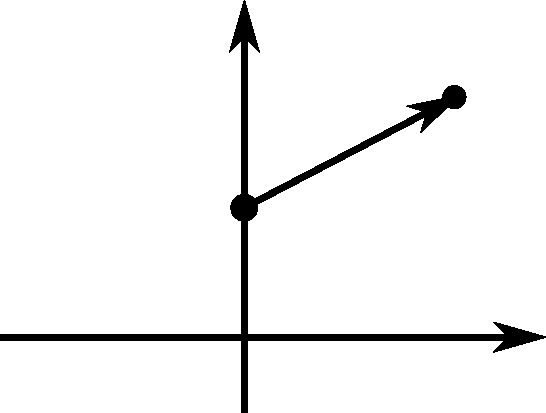
\includegraphics[width=4cm]{3_21 i}
					\wrapincfig{3_21 i}{4cm}
				\end{wrapfigure}
				
				$ \del{r} \Phi \big(2,\frac{\pi}{2} \big) = \begin{pmatrix}
					0\\1
				\end{pmatrix}, \quad \del{\theta} \Phi \big( 2,\frac{\pi}{2} \big) = \begin{pmatrix}
					-2\\0
				\end{pmatrix} $\\
				$ \implies \begin{aligned}[t]
					\bound{\del{r}}{p} &= 0 \cdot \bound{\del{x_1}}{p} + \bound{\del{x_2}}{p}\\
					\bound{\del{\theta}}{p} &= -2 \bound{\del{x_1}}{p}
				\end{aligned} $\\
				$ \implies v $ hat in kartesischen Koordinaten die Darstellung $ \bound{\del{x_2}}{p} + 2 \bound{\del{x_1}}{p} $
			\end{minipage}
		\item $ \Phi(x,y) = \begin{pmatrix}
			x\\p+x^3
			\end{pmatrix} = \begin{pmatrix}
				\tilde{x}\\\tilde{y}
			\end{pmatrix}, p = \begin{pmatrix}
				1\\0
			\end{pmatrix} $\\
			$ \bound{\del{x}}{p}\Phi = \begin{pmatrix}
				1\\3
			\end{pmatrix}, \bound{\del{y}}{p}\Phi = \begin{pmatrix}
				0\\1
			\end{pmatrix} $\\
			$ \implies \begin{aligned}[t]
				\bound{\del{x}}{p} &= \bound{\del{\tilde{x}}}{p} + 3\bound{\del{\tilde{y}}}{p} \neq \bound{\del{\tilde{x}}}{p} \ \text{obwohl } \tilde{x} = x\ \text{ist}\\
				\bound{\del{y}}{p} &= \bound{\del{\tilde{y}}}{p}
			\end{aligned}$
	\end{enumerate}
\end{exmp}

\begin{rem}\label{3.22}
	Beachte: Schreibt man ein Element $v \in T_pM$ als $ v = \sum v_i \bound{\del{x_i}}{p} = \sum \tilde{v}_j \bound{\del{y_j}}{p} $, so gilt also
	\[ \sum_{i=1}^{n} v_i \bound{\del{x_i}}{p} = \sum_{i=1}^{n} v_i \sum_{j=1}^n \frac{\del{\Phi_j}}{\del{x_i}}(\hat{p}) \bound{\del{y_j}}{p}, \]
	\[ \text{Also } \tilde{v}_j = \sum_{i=1}^n \del{x_i} \Phi_j(\hat{p}) v_i\quad \text{"kovariantes Transformationsverhalten"} \]
	Wie transformieren sich Elemente des Kotangentialraums? Sei $w \in T_pM^*$. Bezeichne $ (\bound{\alpha_1}{p},\dotsc, \bound{\alpha_n}{p}) $ die zu $ (\del{x_1},\dotsc, \del{x_n}) $ duale Basis, $ (\bound{\tilde{\alpha}_1}{p},\dotsc, \bound{\tilde{\alpha}_n}{p}) $ die zu $ (\del{y_1},\dotsc, \del{y_n}) $. Dann schreibt sich $w$ als 
	\[ w = \sum w_i \bound{\alpha_i}{p} = \sum \tilde{w}_j \bound{\tilde{\alpha}_j}{p}, \]
	wobei $w_i = w \big( \bound{\del{x_i}}{p} \big)$ und $\tilde{w}_j = w \Big( \bound{\del{y_j}}{p} \Big)$. Somit folgt
	\begin{align*}
		w_i &= w \big( \bound{\del{x_i}}{p} \big) = w \Bigg( \sum_{j=1}^n \underbrace{\del{x_i} \Phi_j(\hat{p})}_{\in \R} \bound{\del{y_j}}{p} \Bigg)\\
		&= \sum_{j=1}^n \del{x_i} \Phi_j(\hat{p}) \tilde{w}_j\quad \text{"kontravariantes Transformationsverhalten"}
	\end{align*}
	Beziehungsweise für die Basis:
	\[ \tilde{\alpha}_j = \sum_{i=1}^n \del{x_i}\Phi_j (\hat{p}) \bound{\alpha_i}{p} \]
\end{rem}
\addtocounter{thm}{1}
\begin{defn}[Differential-Eins-Form]\index{Differentialform}
	Ein glatter Schnitt $M \to T^*M$ heißt \emph{Differential-Eins-Form}. Die Menge der Differentialformen bezeichnet man mit $\Omega^1(M)$. Ist $U \subset M$ offen, so bezeichnet man die Menge der glatten Schnitte $ U \to \bound{T^*M}{U} $ mit $\Omega^1(U)$.
\end{defn}

In Koordinaten: Die Koeffizientenfunktion hängt glatt von $p \in M$ ab:

\begin{exmp*}
	$p \mapsto T_pf,\ f \in C^\infty(M)$, das Differential von $f$ ist $\in \Omega^1(M)$. Man schreibt dafür auch $df$ (anstelle von $p \mapsto T_pf$). Denn:\\
	In Koordinaten gilt $ T_pf \big( \bound{\del{x_i}}{p} \big) = \del{x_i} f(p) $ (denn $T_pf$ ist in dieser Basis die Jacobimatrix!), das heißt $\bound{df}{p}$ lässt sich schreiben als
	\[ \bound{df}{p} = \sum_{i=1}^n \del{x_i} f(p) \bound{\alpha_i}{p} \quad \leftarrow \text{duale Basis zu }\del{x_1},\dotsc, \del{x_n} \]
	Insbesondere gilt für die Koordinatenfunktion $ f = x_j: \bound{dx_j}{p} = \bound{\alpha_j}{p}. $\\
	Diese Notation wollen wir daher im Folgenden für die duale Basis verwenden.
\end{exmp*}

\begin{lem}
	Sei $ (\varphi,U) $ eine Karte von $M$ bei $p \in U$. Dann lässt sich jedes $ \alpha \in \Omega^1(M) $ schreiben als
	\[ \alpha = \sum_{i=1}^n f_i d x^i, \]
	$dx_i \in \Omega^1(U)$, mit $f_i \in C^\infty(U)$ eindeutig bestimmt.
\end{lem}

\begin{exmp*}
	$ \Phi(r,\theta) = \begin{pmatrix}
		r\cos\theta\\ r \sin\theta
	\end{pmatrix} $\\
	$\alpha \in \Omega^1(\R^2) \implies w = f(x,y)dx + g(x,y)dy$, $f$ und $g$ glatt.\\
	Wir könnten die Formel aus \ref{3.22} verwenden,
	\[ \bound{\tilde{\alpha}}{p} = \sum_{i=1}^n \del{x_i} \Phi_j (\hat{p}) \bound{\alpha_i}{p}, \]
	schneller geht es direkt:
	\begin{align*}
		dh &= \sum \del{y_j} h dy^i\\
		d(r\cos\varphi) &= \cos\varphi dr - r \sin\varphi d\varphi\\
		d(r\sin\varphi) &= \sin\varphi dr + r \cos\varphi d\varphi
	\end{align*}
	\begin{align*}
		\implies w &= \Big(f \big(r\cos\theta,r\sin\theta \big)\cos\theta + g \big(r\cos\theta,r\sin\theta \big)\sin\theta\Big) dr\\
		&+ r\Big(-f \big(r\cos\theta,r\sin\theta \big)\sin\theta + g \big(r\cos\theta,r\sin\theta \big)\cos\theta\Big) d\theta
	\end{align*} 
\end{exmp*}
\lecture
\begin{rem*}[Eigenschaften des Differentials]
	$ \lambda,\mu \in \R, f,g \in C^\infty(M) $. Dann gilt:
	\begin{enumerate}[label={\roman*})]
		\item $ d(\lambda f + \mu g)= \lambda df + \mu dg $
		\item $ d(fg) = df \cdot g + f \cdot dg $
		\item $ d(h \circ f) = (h' \circ f)df $ für $ h: I \to \R, h \in C^\infty, I \subset \R $
		\item $ df=0 \iff f $ konstant auf den Zusammenhangskomponenten von $M$.
	\end{enumerate}
\end{rem*}

\begin{rem*}
	Wie in der Diff 2 überlegt man sich, dass $df$ eine lineare Approximation von $f$ ist.
	\image{3_26a}{14cm}
\end{rem*}

\begin{defn}[Ableitung entlang einer Kurve]\index{Ableitung entlang einer Kurve}
	Sei $ \gamma: I \to M $ eine glatte Kurve in $M$ ($M$ differenzierbar, $I \subset \R$ Intervall). Sei $f \in C^\infty(M)$. Dann ist
	\[ (f \circ \gamma)'(t) = df_{\gamma(t)}(\gamma'(t)) \]
	die "\emph{Ableitung von $f$ entlang der Kurve $\gamma$}".
	\image{3_26b}{14cm}
\end{defn}

\begin{rem*}
	$ \bound{df}{p}: T_pM \to \underbrace{T_{f(p)}\R}_{\cong \R} $, also $ \bound{df}{p} \in T_p^*M $\\
	$ (f \circ \gamma)'(t) \in \underbrace{T_{(f \circ \gamma) (t)}\R}_{\cong \R} $, also ist $(f \circ \gamma)'(t)$ die übliche Ableitung.
\end{rem*}

\begin{defn}[Pullback]\index{pullback}
	Sei $ f: M \to N $ (differenzierbare Mannigfaltigkeiten) glatt und $p \in M$. $ \bound{df}{p}: T_pM \to T_{f(p)}N $ legt eine duale Abbildung $ \bound{df}{p}^*: T_{f(p)}^*N \to T_p^*M $ eindeutig fest vermöge
	\[ \bound{df}{p}^*(\underbrace{\omega}_{\in T_{f(p)}^*N})(\underbrace{v}_{\in T_pM}) := \omega(\underbrace{\bound{df}{p}(v)}_{\in T_{f(p)}N}), \]
	$ \bound{df}{p}^* (\omega) \in T_p^*M $, der \emph{"pullback von $\omega$ entlang $f$ bei $p$"}.\\
	Für $\omega \in \Omega^1(N)$ definiert dies einen Schnitt $ f^*\omega: M \to T^*M $ vermöge $ p \mapsto \bound{(f^*\omega)}{p} $ mit
	\[ \bound{f^*\omega}{p} = \bound{df}{p}^* (\underbrace{\omega_{f(p)}}_{\in T_{f(p)}^*N}) \in T_p^*M. \]
\end{defn}

\begin{prop}[Eigenschaften des pullback]
	Ist $ f: M \to N $ glatt, $h \in C(N)$, dann ist
	\[ f^*(h\omega) = (h \circ f) \cdot f^*\omega\quad \foralll \omega \in \Omega^1(N) \]
	Ist $h \in C^\infty(N)$, so ist
	\[ f^*dh = d(h \circ f) \]
\end{prop}

\begin{cor*}
	$ f: M \to N $ glatt, $\omega$ stetiger oder glatter Schnitt in $T^*N$, dann ist $f^*\omega$ ein stetiger oder glatter Schnitt in $T^*M$. Insbesondere also ist $f^*\omega \in \Omega^1(M)$ falls $\omega \in \Omega^1(N)$.
\end{cor*}

\begin{exmp*}
	$ f: \R^3 \to \R^2, f(x_1,x_2,x_3) = \begin{pmatrix}
		x_1x_2^2\\ x_2 \cos(x_3)
	\end{pmatrix} $\\
	$ \omega \in \Omega^1(\R), \omega = y_1dy_2 + y_2dy_1 $
	\begin{align*}
		f^*\omega &= (y_1 \circ f)d(y_2 \circ f) + (y_2 \circ f)d(y_1 \circ f)\\
		&=(x_1x_2^2)d(x_2\cos(x_3)) + (x_2\cos(x_3))d(x_1x_2^2)\\
		&= x_2^3\cos(x_3)dx_1 + 3x_1x_2^2\cos(x_3)dx_2 - x_1x_2^3\sin(x_3)dx_3
	\end{align*}
\end{exmp*}

\begin{rem*}
	Genauso kann man auch Koordinatenwechsel als pullback entlang der Identitätsabbildung $M \to M$ sehen, wobei einmal Koordinaten $(\varphi,U)$ und einmal Koordinaten $(\psi,V)$ bei $p \in M$ gewählt werden:
\end{rem*}

\begin{exmp*}
	Polarkoordinaten in $\R^2$
	\begin{align*}		
		\omega &= xdy \ \text{(in kartesischen Koordinaten)}\\
		&= \id^*(xdy) = r\cos\theta d(r\sin\theta)
	\end{align*}
\end{exmp*}

Es ist kein Zufall, dass wir Differentialformen $dx_i$ notieren (in Koordinaten). Betrachte etwa $ \omega \in \Omega^1(\R), \bound{\omega}{t} = \omega_1(t)dt. $ Man definiert $ \int_{[a,b]}\omega := \int_a^b \omega_1(t)dt $ als das \emph{"Integral über $\omega$"}.\\
Diese Definition ist sinnvoll, wenn wir zeigen, dass sie nicht von der Wahl der Koordinaten abhängt:

\begin{lem}
	Sei $ \omega \in \Omega^1([a,b]) $. Sei $ \varphi:[c,d] \to \R,\ \varphi([c,d]) = [a,b], $ ein Diffeomorphismus mit $\varphi' > 0$ auf $[c,d]$ (also monoton wachsend), dann ist
	\[ \int_{[c,d]} \varphi^*\omega = \int_{[a,b]} \omega. \]
	Ist $\varphi$ monoton fallend, so gilt
	\[ \int_{[c,d]} \varphi^*\omega = - \int_{[a,b]} \omega. \]
\end{lem}

\begin{defn}[Kurvenintegral]\index{Kurvenintegral}
	Sei $ \gamma: [a,b] \to M $ ein glattes Kurvenstück (Glattheit in $a,b$ wie in Diff 1) und $\omega \in \Omega^1(M)$. Dann definiert man das \emph{Kurvenintegral} von $\omega$ entlang $\gamma$ als
	\[ \int_\gamma \omega = \int_{[a,b]} \gamma^*\omega. \]
	Ist $\gamma$ stückweise glatt, gibt es also eine endliche Partition von $[a,b], a=a_0 < \dots < a_n = b,$ sodass $\bound{\gamma}{[a_i,a_{i+1}]}$ glatt ist, so definiert man es als 
	$$ \int_{\gamma} \omega = \sum_{i=1}^{n} \int_{[a_{i-1},a_i]} \gamma^*\omega. $$
\end{defn}

\begin{lem}
	Sei $M$ eine differenzierbare Mannigfaltigkeit und $\gamma: [a,b] \to M$ glatt. Dann gilt
	\begin{enumerate}[label={\roman*})]
		\item $ \int_\gamma (\lambda \omega + \mu \eta) = \lambda \int_\gamma \omega + \mu \int_\gamma \eta \quad \foralll \omega,\eta \in \Omega^1(M), \ \foralll \lambda,\mu \in \R $
		\item Ist $\gamma$ konstant, so ist $ \int_\gamma \omega = 0 \quad \foralll \omega \in \Omega^1(M) $.
		\item $ \gamma_1 = \bound{\gamma}{[a,c]}, \gamma_2 = \bound{\gamma}{[c,b]}, a \leq c \leq b $\\
			$ \implies \int_\gamma \omega = \int_{\gamma_1} \omega + \int_{\gamma_2} \omega\quad \foralll \omega \in \Omega^1(M) $
		\item Ist $ f: M \to N $ glatt und $\eta \in \Omega^1(N)$, so ist
		\[ \int_\gamma \underbrace{f^*\eta}_{\in \Omega^1(M)} = \int_{f \circ \gamma} \eta. \]
	\end{enumerate}
\end{lem}

\begin{exmp*}
	$ M = \R^2 \setminus \{0\},\ \omega = \frac{1}{x^2+y^2}(xdy-ydx),\ \gamma: [0,2\pi] \to M, \gamma(t) = (\cos t,\sin t)^T $\\
	\[ \int_\gamma \omega = \int_{[0,2\pi]} \Big( (\cos t)^2 dt - \big(-(\sin t)^2 \big) dt \Big) = \int_0^{2\pi} dt = 2\pi \]
\end{exmp*}

Das Kurvenintegral hängt nicht von der Parameter-Beschreibung der Kurve ab:

\begin{lem}
	Sei $ \gamma: [a,b] \to M $ eine stückweise glatte Kurve, dann heißt $ \tilde{\gamma}: [c,d] \to M $ \emph{Reparametrisierung} von $\gamma$ (unter Beibehaltung der Umlaufrichtung bzw. unter Umkehr der Umlaufrichtung), falls es einen Diffeomorphismus $\varphi: [a,b] \to [c,d]$ gibt (mit $\varphi' > 0$ bzw. $\varphi' < 0$ auf $(a,b)$). Ist $\omega \in \Omega^1(M)$, so gilt
	\[ \int_\gamma \omega = \pm \int_{\tilde{\gamma}} \omega. \]
	\begin{itemize}
		\item[$+$] falls $\tilde{\gamma}$ Reparametrisierung von $\gamma$ der selben Umlaufrichtung ist,
		\item[$-$] falls $\tilde{\gamma}$ Reparametrisierung von $\gamma$ der umgekehrten Umlaufrichtung ist.
	\end{itemize}
\end{lem}

\begin{rem*}
	Es gilt $ \int_\gamma \omega = \int_a^b \omega_{\gamma(t)} (\gamma'(t))dt, $ denn wenn $\gamma$ ganz in einem Kartenbereich verläuft gilt (für $\gamma$ glatt):
	\begin{align*}
		\omega_{\gamma(t)} (\gamma'(t)) &= \sum \omega_i (\gamma(t)) dx_i (\gamma'(t))
			= \sum \omega_i(\gamma(t)) \gamma_i' (t)\\
		\implies \bound{(\gamma^*\omega)}{t} &= \sum \omega_i (\gamma(t)) \bound{d\gamma_i}{t}
			= \underbrace{\sum \omega_i (\gamma(t)) \gamma_i'(t)}_{\omega_{\gamma (t)}} dt
	\end{align*}
	Verläuft $\gamma$ nicht in einem einzigen Kartenbereich, so gibt es eine Partition $ a=\tilde{a}_0 < \dots < \tilde{a}_n = b $, sodass $ \bound{\gamma}{[\tilde{a}_i,\tilde{a}_{i+1}]} $ jeweils in einem Kartenbereich verläuft. Dann sei $ \gamma([a,b]) \subset \bigcup_{j \in J} U_j $, dann gibt es $ j_1,\dotsc,j_k$, sodass $ \underbrace{\gamma([a,b])}_{kompakt!} \subset U_{j_1} \cup \dots \cup U_{j_k}. $\\
	Für stückweise glatte Kurven betrachtet man jeweils glatte Einschränkungen $ \bound{\gamma}{[a_{i-1},a_i]}. $
\end{rem*}

\begin{thm}\label{3.33}
	Sei $ f \in C^\infty(M) $ und $ \gamma:[a,b] \to M $ stückweise glatt. Dann gilt
	\[ \int_\gamma df = f(\gamma(b)) - f(\gamma(a)). \]
\end{thm}
\begin{defn}[Exakte Differentialform]\index{Differentialform!exakte}\lecture
	$ \alpha \in \Omega^1(M) $ heißt \emph{exakt}, falls es $f \in C^\infty(M)$ gibt, sodass $ \alpha = df $. In dem Fall heißt $f$ ein \emph{Potential} für $\alpha$.
\end{defn}

\begin{rem*}
	\begin{enumerate}[label={\roman*})]
		\item Nicht jede Form ist exakt!
		\item Potentiale sind nicht eindeutig: $ df = d(f+c) $ für jede konstante Funktion $c$.
		\item Nach Satz \ref{3.33} gilt: Ist $\alpha \in \Omega^1(M)$ exakt, so ist das Integral
			\[ \int_\gamma \alpha = f(\gamma(b)) - f(\gamma(a)) \]
			wenn $\gamma: [a,b] \to M$ stückweise glatt ist.
	\end{enumerate}
\end{rem*}

\begin{defn}[Konservative Differentialform]\index{Differentialform!konservative}
	$ \alpha \in \Omega^1(M) $ heißt \emph{konservativ}, falls $ \int_\gamma \alpha = 0 $ für alle geschlossenen stückweise glatten Kurven $ \gamma: [a,b] \to M $, für die also gilt $\gamma(a) = \gamma (b)$.
\end{defn}

\begin{thm}
	Folgende Aussagen sind für $ \alpha \in \Omega^1(M) $ äquivalent:
	\begin{enumerate}[label={\roman*})]
		\item $\alpha$ ist konservativ.
		\item $\int_\gamma \alpha = \int_{\tilde{\gamma}} \alpha$ für alle stückweise glatten Kurven $ \gamma: [a,b] \to M, \tilde{\gamma}: [c,d] \to M $ mit $ \gamma(a) = \tilde{\gamma}(c), \gamma(b) = \tilde{\gamma}(d). $ (Wegunabhängigkeit)
		\item $\alpha$ ist exakt.
	\end{enumerate}
\end{thm}

\begin{rem*}
	Oft ist es leichter, ein Potential zu raten.
	\begin{exmp*}
		$\omega = y\cos(xy) dx + x\cos(xy)dy, f = \sin(xy)$
	\end{exmp*}
\end{rem*}

\begin{defn}[Geschlossene Differentialform]\index{Differentialform!geschlossene}
	Sei $ \alpha \in \Omega^1(M) $ und $q_0 \in M$. Gilt in einer (und somit in jeder) Karte $ (\varphi,U)$ bei $ q_0 $
	\[ \del{x_i} \alpha_j (q) = \del{x_j} \alpha_i(q) \qquad \foralll q \in U,\ \foralll i,j \in \{1,\dotsc,n\}, \]
	so nennt man $\alpha$ \emph{geschlossen}.
\end{defn}

\begin{rem*}
	Jede exakte Form ist geschlossen. (Satz von Schwarz)
\end{rem*}

\begin{lem}
	$\omega$ ist geschlossen $\iff \ \foralll U \subset M$ offen und für alle Vektorfelder $X,Y: U \to TU$ (wie immer: glatte Schnitte) gilt:
	\[ X(\omega(Y)) - Y(\omega(X)) = \omega([X,Y]), \]
	wobei $[X,Y] = X \circ Y - Y \circ X$ der "Kommutator" ist.
\end{lem}

\begin{rem*}
	Zunächst stellen wir fest, dass gilt $ [X_p,Y_p] \in T_pM: $
	\begin{align*}
		\sum X_i(p) \bound{\del{i}}{p} Y_j(p) \bound{\del{j}}{p} -& \sum Y_i(p) \bound{\del{i}}{p} X_j(p) \bound{\del{j}}{p} = \\
		=&\sum_{i,j} X_i(p) \del{i} Y_j(p) \bound{\del{j}}{p} + \sum_{i,j} X_i(p) Y_j(p) \bound{\del{i} \del{j}}{p}\\
		&- \sum_{i,j} Y_j(p) \del{j} X_i(p) \bound{\del{i}}{p} + \sum_{i,j} Y_j(p) X_i(p) \bound{\del{j} \del{i}}{p}\\
		=& \sum_{i,j} X_i(p) \del{i} Y_j(p) \bound{\del{j}}{p} - \sum_{i,j} Y_j(p) \del{j} X_i(p) \bound{\del{i}}{p}
	\end{align*}
\end{rem*}

\begin{rem}
	Ist $ f: M \to N $ ein lokaler Diffeomorphismus (d.h. zu $p \in M \ \existss U \subset M, p \in U,$ und $V \subset N$, sodass $ \bound{f}{U}: U \to V $ ein Diffeomorphismus ist, also glatt mit glatter Umkehrfunktion), so bildet $f^*$ exakte Formen auf exakte Formen ab und geschlossene auf geschlossene.
\end{rem}

\begin{thm}[Lemma von Poincaré]\label{3.40}
	\begin{minipage}{\linewidth}
		\begin{wrapfigure}{R}{5cm}
			\centering
			\wrapincfig{3_40}{3cm}
		\end{wrapfigure}
		
		Ist $ U \subset \R^n $ sternförmig (d.h. $\existss p_0 \in U$, sodass alle geraden Verbindungsstrecken von $p_0$ zu beliebigen Punkten $p$ ganz in $U$ enthalten sind), dann ist jede geschlossene Form auf $U$ exakt.
	\end{minipage}
\end{thm}

\begin{exmp*}
	Die geschlossene, auf $\R^2 \setminus \{0\}$ nicht exakte Form $ \alpha = \frac{1}{x^2+y^2}(ydx-xdy) $ ist auf $ \{(x,y) \in \R^2 \mid x > 0\} $ exakt ($ f = \tan^{-1} \frac{y}{x} $)
\end{exmp*}

\begin{cor}
	Ist $ \omega \in \Omega^1(M)$ geschlossen, so besitzt jeder Punkte $ p \in M $ eine Umgebung, auf der $\omega$ exakt ist.
\end{cor}
	\chapter{Tensorfelder}
\lecture

\begin{rem}
	Erinnerung an \ref{3.18}: Tensorprodukt zweier Bündel $ (E, \pi_E, B), (F, \pi_F,B)$, $E \otimes F = \bigcup_{x \in B} E_x \otimes F_x, (E \otimes F)_x := E_x \otimes F_x. $\\
	Sind $ (\varphi_E,U) $ und $(\varphi_F,U)$ Bündelkarten, $ \varphi_E: \pi_E^{-1}(U) \to U \times \R^n, \varphi_F: \pi_F^{-1}(U) \to U \times \R^m, $ so ist
	\[ \varphi_E \otimes \varphi_F: \underbrace{\pi_E^{-1}(U) \otimes \pi_F^{-1}(U)}_{= \pi^{-1}(U)} \to U \times (\R^n \otimes \R^m) \]
	\[ \bound{\varphi_E \otimes \varphi_F}{x}(E_x \otimes F_x) = \{x\} \times (\R^n \otimes \R^m) \]
	eine Bündelkarte für $E \otimes F$. Die Topologie auf $E \otimes F$ wählt man wieder so, dass $\varphi_E \otimes \varphi_F$ ein Homöomorphismus ist.
\end{rem}

\begin{rem*}
	Hier ist wichtig, dass $ \bound{\varphi_E}{x} \otimes  \bound{\varphi_F}{x} $ stetig von $ \bound{\varphi_E}{x} $ und $ \bound{\varphi_F}{x} $ abhängt, denn nach Basiswechsel erhält man Matrizen, und
	\[ A \otimes B = \begin{pmatrix}
		a_{11}B & \cdots & a_{1n}B\\
		a_{21}B & 		& \vdots\\
		\vdots &	&\\
		a_{n1}B & \cdots & a_{nn}B
	\end{pmatrix} \]
	(Bei der direkten Summe war das (hoffentlich) unmittelbar klar...)
\end{rem*}

\begin{defn}[Tensorprodukt, äußere Potenz]\index{Tensorprodukt}\index{äußere Potenz}
	Das \emph{$k$-fache Tensorprodukt} von $ (E,\pi,B) $ ist
	\[ E^{\otimes k} := \bigcup_{x \in B} (E_x)^{\otimes k}. \]
	Mit Karten $(\varphi,U)$ von $E$ haben wir als Karten von $E^{\otimes k}$ $(\varphi^{\otimes k},U)$ mit
	\[ \bound{\varphi^{\otimes k}}{x} (v_1 \otimes \dots \otimes v_k) = \bound{\varphi}{x}(v_1) \otimes \dots \otimes \bound{\varphi}{x}(v_k) \]
	\[ \bound{\varphi^{\otimes k}}{x}: E_x^{\otimes k} \to \{x\} \times (\underbrace{\R^n \otimes \dots \otimes \R^n}_{k\text{-fach}}) \]
	Die \emph{$k$-fache äußere Potenz} von $(E,\pi,B)$ ist
	\[ \Lambda^k E:= \bigcup_{x \in B} \Lambda^k(E_x) \]
	\[ \Lambda^k(V) := V_1 \otimes \dots \otimes V_k / R, \]
	\[ R = \Span\{v_1 \otimes \dots \otimes v_k - \sgn(\sigma) v_{\sigma(1)} \otimes \dots \otimes v_{\sigma(k)} \mid v_j \in V_j, \sigma \in \Sigma_k\} \]
	Die Karten $(\Lambda^k\varphi,U)$ für Karten $(\varphi,U)$ von $E$ sind
	\[ \Lambda^k\varphi = \varphi^{\otimes k}/R. \]
\end{defn}

\begin{rem*}
	Das Tensorprodukt selbst kann man sehr abstrakt einführen, aber wir werden meist mit Basen arbeiten, da wir uns für folgende Situation interessieren:
\end{rem*}

\begin{defn}[Tensorbündel, Tensorfeld, $k$-Form]\index{Tensorbündel}\index{Tensorfeld}\index{Differentialform}
	\begin{enumerate}[label= {\roman*})]
		\item Das \emph{Tensorbündel} von Grad $(k,l)$ über einer differenzierbaren Mannigfaltigkeit $M$ ist das Bündel
			\[ T^{(k,l)} TM := \bigcup_{p \in M} \big(T_pM\big)^{\otimes k} \otimes \big(T_p^*M\big)^{\otimes l}, \]
			mit $k,l \in \N_0$. $(T_pM)^{\otimes k}$ nennt man "kontravariante Tensoren" $k$-ter Stufe, $(T_p^*M)^{\otimes l}$ "kovariante Tensoren" $l$-ter Stufe.\hspace{\fill} $ (V^{\otimes 0} = \R, \R \otimes W = W) $\\
			Notation: $ T^{(k,0)} TM = T^k(TM), T^{(0,l)}TM = T^l(T^*M) $\\
			Ein Schnitt in einem solchen Bündel heißt (kontra-/kovariantes oder gemischtes) \emph{Tensorfeld} auf $M$.
		\item Ein glatter Schnitt in der $k$-fachen äußeren Potenz von $T^*M$,
			\[ \Lambda^kT^*M = \bigcup_{p \in M} \Lambda^k \big(T_p^*M\big), \]
			heißt \emph{Differentialform} vom Grad $k$ auf $M$.
	\end{enumerate}
\end{defn}

\begin{rem*}
	In lokalen Koordinaten:\\
	$A$ Schnitt in $T^{(k,l)}TM:$
	\[ \bound{A}{p} = \sum A_{i_1\dots i_l}^{j_1\dots j_k} \bound{\del{j_1}}{p} \otimes \dots \otimes \bound{\del{j_k}}{p} \otimes \bound{dx^{i_1}}{p} \otimes \dots \otimes \bound{dx^{i_l}}{p} \]
	$\omega$ Differentialform von Grad $k$:
	\[ \bound{\omega}{p} = \sum_{i_1 < \dots < i_k} \omega _{i_1\dots i_k} dx^{i_1} \wedge \dots \wedge dx^{i_k} \]
	Jeweils mit \emph{glatten} Koeffizienten $ p \mapsto A_{i_1\dots i_l}^{j_1\dots j_k}(p) \in \R, p \mapsto \omega_{i_1\dots i_k}(p) $
\end{rem*}

\begin{lem}
	Seien $ V_1,\dotsc,V_k $ endlich-dimensionale Vektorräume. Seien $ (v_{1,1}, \dotsc, v_{1,n_1})$, $(v_{2,1}, \dotsc, v_{2,n_2})$, $\dotsc, (v_{k,1}, \dotsc, v_{k,n_k}) $ Basen von $V_1,V_2,\dotsc,V_k$. Dann ist
	\[ \big\{ v_{1,j_1} \otimes v_{2,j_2} \otimes \dots \otimes v_{k,j_k} \mid 1 \leq j_i \leq n_i \big\} \]
	eine Basis von $V_1 \otimes \dots \otimes V_k$ mit Dimension $n_1 \dotsm n_k$. Ist $V$ ein endlich-dimensionaler Vektorraum, $ (v_1,\dotsc,v_n) $ eine Basis von $V$, so ist
	\[ \big\{ v_{i_1} \wedge v_{i_2} \wedge \dots \wedge v_{i_k} \mid i_1 < \dots < i_k,\ i_1,\dotsc,i_k \in \{1,\dotsc,n\} \big\} \]
	eine Basis von $\Lambda^kV$ mit Dimension $\binom{n}{k}$.
\end{lem}

Hierbei ist das Dachprodukt $\wedge$ wie folgt definiert:
\[ \wedge: \Lambda^ V \times \Lambda^l V \to \Lambda^{k+l} V \]
\[ a \wedge b = \frac{(k+l)!}{k!l!} Alt_{k+l} (a\otimes b),\ \text{wobei} \]
\[ Alt_m (\underbrace{c_1 \otimes \dots \otimes c_m}_{\in T^mV}) = \frac{1}{m!} \sum_{\sigma \in \Sigma_m} \sgn(\sigma) (c_{\sigma(1)} \otimes \dots \otimes c_{\sigma(m)}) \]
und lineare Fortsetzung auf beliebige $c \in T^m V$ ("Antisymmetrierungs-Abbildung")

\begin{rem}
	\begin{enumerate}[label={\roman*})]
		\item Kovariante Tensoren $ \in T^l(T_p^*M) $ fassen wir auch als multilineare Abbildungen
			\[ \underbrace{T_pM \times \dots \times T_pM}_{l\text{-fach}} \to \R \]
			auf. Denn es gilt allgemein (für $\dim(V_j)<\infty$):
			\[ V_1^* \otimes \dots \otimes V_l^* \cong \{ \text{Multilineare Abbildungen } V_1 \times \dots \times V_l \to \R \} =: \Lcal. \]
		\item Somit gilt (wegen $V^{**} = V$ kanonisch)
			\[ V_1 \otimes \dots \otimes V_k \cong \{ \text{Multilineare Abbildungen } V_1^* \times \dots \times V_k^* \to \R \}. \]
	\end{enumerate}
\end{rem}

\begin{exmp*}
	$ M = \R^4 $, kartesische Koordinaten
	\[ \bound{A}{x} = A_{13}^2(x) \del{x_2} \otimes dx^1 \otimes dx^3 + A_{14}^2(x) \del{x_2} \otimes dx^1 \otimes dx^4 \]
	\[ \bound{A}{x} : T_x^*\R^4 \otimes T_x\R^4 \otimes T_x\R^4 \to \R \]
	\begin{align*}
		\bound{A}{x} &\Big( \big(\alpha_1(x) dx^1 + \alpha_2(x) dx^2\big) \otimes \big(f^1(x)\del{x_1} + f^3(x)\del{x_3}\big) \otimes \big(g(x) \del{x_3}\big) \Big) \\&= A_{13}^2(x) \alpha_2(x) f^1(x) g(x) + 0
	\end{align*}
	$ \bound{\omega}{x} \in \Lambda^3 T_x^*\R^4 (\cong \Lambda^3 \R^4) $. Allgemeinste Form:
	\begin{align*}
		\bound{\omega}{x} &= \omega_{123} dx^1 \wedge dx^2 \wedge dx^3\\
		&+ \omega_{124} dx^1 \wedge dx^2 \wedge dx^4\\
		&+ \omega_{134} dx^1 \wedge dx^3 \wedge dx^4\\
		&+ \omega_{234} dx^2 \wedge dx^3 \wedge dx^4
	\end{align*}
\end{exmp*}

\begin{lem}
	Sei $ A $ ein $C^\infty$-Schnitt in $T^{(k,l)}(TM)$, $B$ ein $C^\infty$-Schnitt in $T^{\left(\bar{k},\bar{l}\right)}(TM)$, $f \in C^\infty(M)$. Dann ist $ fA $ ein $C^\infty$-Schnitt in $T^{(k,l)}(TM)$ und $ A \otimes B $ ein $C^\infty$-Schnitt in $T^{\left(k + \bar{k},l + \bar{l}\right)}(TM)$ mit Komponentenfunktionen
	\[ f(p)A_{j_1\dots j_l}^{i_1\dots i_k}(p) \quad \text{bzw.} \quad
	(A \otimes B)_{j_1\dots j_{l+\bar{l}}}^{i_1\dots i_{k+\bar{k}}}(p) = A_{j_1\dots j_l}^{i_1\dots i_k} B_{j_{l+1}\dots j_{l+\hat{l}}}^{i_{k+1}\dots i_{k+\hat{k}}}(p) \]
\end{lem}

\begin{rem*}
	Ein $C^\infty$-Schnitt in $T^k(T^*M)$ ($ = T^{(0,k)}(TM) $) $A$ induziert mit Vektorfeldern $\Xfrak$ ($\cong T^{(1,0)}(TM)$) eine multilineare Abbildung
	\[ \Acal: \Xfrak(M) \times \dots \times \Xfrak(M) \to C^\infty(M) \]
	(multilinear wegen der Definition des Tensorprodukts)\\
	Diese Abbildung ist sogar $C^\infty (M)$-multilinear, also
	\[ \Acal \big( X_1,\dotsc, fX_j + g\tilde{X}_j,\dotsc \big) = f\Acal (\dotsc,X_j,\dotsc) + g\Acal(\dotsc,\tilde{X}_j,\dotsc) \quad \foralll j,\ \foralll f,g \in C^\infty(M) \]
	Es gilt auch die Umkehrung:
\end{rem*}

\begin{lem}\label{4.7}
	Eine Abbildung 
	\[ \Acal: \underbrace{\Xfrak(M) \times \dots \times \Xfrak(M)}_{k\text{-mal}} \to C^\infty(M) \]
	wird genau dann von einem Tensorfeld ($k$-ter Stufe) induziert, wenn $\Acal$ $C^\infty(M)$-multilinear ist.
\end{lem}

\subsection*{Einschub zum Tensorprodukt (Wiederholung AGLA)}
	Ebenso wie die direkte Summe kann man auch das Tensorprodukt über eine universelle Eigenschaft charakterisieren. Zunächst seien $V_1,\dotsc,V_k$ endlich-dimensionale Vektorräume.
	\begin{align*}
		V_1 \otimes \dots \otimes V_k &= \vertarrowbox[1ex]{\Fcal}{freier Vektorraum} (V_1 \times \dots V_k)/\sim\\
		&= \big\{ f: v_1 \times \dots \times v_k \to \R \mid f(x) = 0\ \text{nur für endlich viele } x \in V_1 \times \dots \times V_k \big\}\\
		&= \Bigg\{ f = \sum_{j=1}^N \lambda_j \delta_{x_j} \mid N \in \N, \lambda_j \in \R, x_j \in V_1 \times \dots \times V_k \Bigg\}\\
		\text{mit }\delta_{x_j}(x) &= \begin{cases}
				1 \quad &x=x_j,\\0 \quad &\text{sonst.}
			\end{cases}
	\end{align*}
	Man identifiziert $\delta_x$ mit $x$, sodass $V_1 \times \dots \times V_k \subset \Fcal$
	\begin{prop*}
		Ist $ L: V_1 \times \dots \times V_k \to W $ ($W$ Vektorraum) multilinear, das heißt linear in jedem Eintrag $V_j$, dann gibt es eine eindeutig bestimmte lineare Abbildung $ l: V_1 \otimes \dots \otimes V_k \to W $, sodass
		\[ \begin{tikzcd}
			V_1 \times \dots \times V_k \arrow{r}{L} \arrow{d}{Proj.} & W\\
			V_1 \otimes \dots \otimes V_k \arrow{ur}{l}
		\end{tikzcd} \quad \text{kommutiert.} \]
	\end{prop*}
	\chapter{Topologisches, Teilung der Eins, Fortsetzungslemmata}
\lecture

\begin{lem}
	Eine topologische Mannigfaltigkeit ist \emph{lokal kompakt}, das heißt $ \foralll p \in  M \ \existss $ offene Umgebung $U$, sodass $ U \subset K $, $K \subset M$ kompakt.
\end{lem}

\begin{rem}\label{5.2}
	Es gibt sogar eine abzählbare Basis der Topologie durch solche präkompakten\footnote{d.h. der Abschluss ist kompakt}  "Koordinatenbälle" (Betrachte $ B_r(q) \ni \hat{q}, r \in \Q, q \in \Q^n $)
\end{rem}

\begin{lem}
	Jeder lokal kompakte topologische Raum $X$ mit abzählbarer Basis der Topologie (insbesondere also eine topologische Mannigfaltigkeit) besitzt eine \emph{Ausschöpfung} durch kompakte Mengen. ($X = \bigcup K_j, K_j \subset \dot{K}_{j+1}, K_j$ kompakt)
\end{lem}

\begin{defn*}[lokal endlich]\index{lokal endlich}
	Sei $\Lcal$ eine Familie von Teilmengen einer topologischen Mannigfaltigkeit $M$. $\Lcal$ heißt \emph{lokal endlich}, falls $ \foralll p \in M \ \existss $ offene Umgebung $U$, sodass $ U \cap L \neq \emptyset $ nur für endlich viele $L \in \Lcal$.
\end{defn*}

\emph{Nicht} lokal endlich: $ \Lcal = \{(-n,n) \subset \R \mid n \in \N_0\} $
\image{5_3}{0.8\textwidth}

\begin{defn*}[Verfeinerung]\index{Verfeinerung}
	Seien $ M = \bigcup_{\alpha \in A} U_\alpha, M = \bigcup_{\beta \in B} V_\beta $ offene Überdeckungen. Dann heißt $ \Vcal = \{V_\beta \mid \beta \in B\} $ \emph{Verfeinerung} von $ \Ucal = \{U_\alpha \mid \alpha \in A\} $, falls $ \foralll V \in \Vcal \ \existss U \in \Ucal $ mit $ V \subset U $.
	\image{5_3b}{0.25\textwidth}
\end{defn*}

\begin{thm}
	Eine topologische Mannigfaltigkeit ist stets \emph{parakompakt}, das heißt jede offene Überdeckung von $M$ besitzt eine lokal endliche Verfeinerung.
\end{thm}

\begin{rem}
	Wir betrachten im Folgenden differenzierbare Mannigfaltigkeiten. Aus Bemerkung \ref{5.2} erhält man:\\
	Jede differenzierbare Mannigfaltigkeit besitzt einen abzählbaren glatten Atlas mit Koordinatenbällen $ \varphi^{-1}\big(B_r(q)\big) \subset M. $
\end{rem}

\begin{defn*}[Zerlegung der Eins]\index{Zerlegung der Eins}
	Sei $ \Ucal $ eine offene Überdeckung von $M$, $M = \bigcup_{\alpha \in A} U_\alpha$. Eine \emph{$\Ucal$ untergeordnete glatte Zerlegung der Eins} ist eine Familie von Funktionen $ \{\psi_\alpha \mid \alpha \in A\}, $ $ \psi_\alpha: M \to \R $ glatt mit
	\begin{enumerate}[label={\roman*})]
		\item $ 0 \leq \psi_\alpha(p) \leq 1 \quad \foralll p \in M $
		\item $ \supp \psi_\alpha \subset U_\alpha \quad \foralll \alpha \in A $
		\item $ \{\supp \psi_\alpha \mid \alpha \in A\} $ ist lokal endlich
		\item $ \sum_{\alpha \in A} \psi_\alpha (p) = 1 \quad \foralll p \in M $
	\end{enumerate}
	$ \sum_{\alpha \in A} $ ist dabei wohldefiniert, da wegen iii) nur endlich viele Beiträge zur Summe $\neq 0$ sind.
	\image{5_4}{0.8\textwidth}
\end{defn*}

\begin{thm}
	Ist $M$ eine differenzierbare Mannigfaltigkeit und $ \Ucal = \{U_\alpha \mid \alpha \in A\} $ eine offene Überdeckung von $M$, dann gibt es eine glatte, $\Ucal$ untergeordnete Zerlegung der Eins.
\end{thm}


\lecture
\begin{lem}
	Ist $ A \subset M $ ($M$ differenzierbare Mannigfaltigkeit) abgeschlossen und $U \supset A$ offen, dann gibt es eine glatte Funktion $\psi: M \to \R$, sodass
	\[ \supp \psi \subset U,\ \bound{\psi}{A} = 1,\ 0 \leq \psi(p) \leq 1 \quad \forall p \in M \]
	("bump function (Höckerfunktion) für $A$ mit Träger in $U$")
\end{lem}

\begin{lem}[Fortsetzungslemma für glatte Funktionen]
	Sei $A \subset M$ abgeschlossen, $ f: A \to \R $ glatt. Dann gibt es zu $U$ offen, $A \subset U$, eine glatte Funktion $\tilde{f}: M \to \R$ mit $ \supp \tilde{f} \subset U $ und $ \bound{\tilde{f}}{A} = f $. $\tilde{f}$ heißt dann eine \emph{"Fortsetzung"} von $f$.
\end{lem}

\begin{rem*}
	\begin{enumerate}[label={\roman*})]
		\item $f$ glatt auf $A$: wenn $\exists$ für jedes $p \in A$ eine offene Umgebung $W_p$ und eine glatte Fortsetzung $ \tilde{f}_p: W_p \to \R,\ \bound{\tilde{f}_p}{W_p \cap A} = \bound{f}{W_p\cap A} $
		\item Ist $A$ nicht abgeschlossen gilt die Aussage nicht unbedingt. Z.B. $ f:(0,1) \to \R, f(x) = \frac{1}{x} $ besitzt keine glatte (nicht einmal eine stetige) Fortsetzung auf $U = (-\epsilon,1),\ \epsilon > 0$.
	\end{enumerate}
\end{rem*}

\begin{rem*}
	Achtung: $f$ wie oben muss Werte in $\R$ (bzw. $\R^k$) annehmen. Es kann sonst topologische Gründe geben, weshalb keine glatten (nicht einmal stetige) Fortsetzungen existieren:\\
	$ A = \Sbb^1 \subset \R^2, f: \Sbb^1 \to \Sbb^1, f(x) = x \ \foralll x \in \Sbb^1 $\\
	$f$ besitzt keine glatte Fortsetzung $ \tilde{f}: \R^2 \to \Sbb^1 $ (nicht einmal eine stetige)
\end{rem*}

\begin{lem}
	Ist $ A \subset M $ abgeschlossen und $X$ ein glattes Vektorfeld entlang $A$, also $ X_p \in T_pM \ \foralll p \in A $ und $\foralll p \in A \ \existss V_p$ offene Umgebung und $ \bound{\tilde{X}}{V_p} $ Vektorfeld (insb. glatt) und $\bound{\tilde{X}}{A} = X$.\\
	Dann $\exists$ Vektorfeld (insb. glatt) auf $M$, das auf $A$ mit $X$ übereinstimmt und so gewählt werden kann, dass es in $U$ getragen ist, $U \supset A$ offen.
\end{lem}
	\chapter{Riemannsche Metrik}

Ein spezielles Tensorfeld auf eine differenzierbaren Mannigfaltigkeit.

\begin{defn*}[Riemannsche Metrik]\index{Riemannsche Metrik}
	Eine \emph{Riemannsche Metrik} ist ein kovariantes Tensorfeld 2. Stufe $g$, das symmetrisch und positiv definit ist, also
	\[ g_p(X_p,Y_p) = g_p(Y_p,X_p) \qquad \foralll p \in M,\ \foralll X_p,Y_p \in T_pM, \]
	\[ g_p(X_p,X_p) > 0 \qquad \foralll p \in M,\ \foralll X_p \neq 0 \in T_pM. \]
\end{defn*}

\begin{rem*}
	\begin{enumerate}[label= {\roman*})]
		\item In lokalen Koordinaten gilt $ g = \sum g_{ij} dx^i \otimes dx^j $ mit $g_{ij}(p)$ symmetrisch.
		\item $ dx^idx^j := \frac{1}{2}(dx^i \otimes dx^j + dx^j \otimes dx^i) $. Dann
			\begin{align*}
				g &= \sum g_{ij} dx^i \otimes dx^j\\
				&= \frac{1}{2} \sum g_{ij} dx^i \otimes dx^j + \frac{1}{2} \sum g_{ji} dx^j \otimes dx^i\\
				&= \sum g_{ij} dx^idx^j
			\end{align*}
		\item $ g_p(v,w) =: \bound{\langle v,w\rangle_g}{p} $ definiert eine innere, positiv definite Form $ T_pM \times T_pM \to \R $
	\end{enumerate}
\end{rem*}

\begin{exmp*}
	Euklidische Metrik: $M = \R^n$
	$ g = (dx^1)^2 + \dots + (dx^n)^2 $
	$ g_p(v,w) = \bound{\langle v,w\rangle_g}{p} = \sum v_jw_j $ wenn $ v = \sum v_j \bound{\del{j}}{p}, w = \sum w_j \bound{\del{j}}{p}$
\end{exmp*}

\begin{rem}\label{6.1}
	Positive Definitheit ist ein von der Wahl der Basis unabhängiges Konzept. Nach dem Trägheitssatz von Sylvester gibt es in $T_pM$ stets eine Basiswahl, sodass
	\[ \bound{(g_{i,j})}{p} = \begin{pmatrix}
		1 & &\\
		& \ddots &\\
		&&1
	\end{pmatrix} \]
\end{rem}

\begin{defn}[Produkt-Metriken]\index{Riemannsche Mannigfaltigkeit}
	Seien $ (M,g) $ und $ (\tilde{M},\tilde{g}) $ \emph{Riemannsche Mannigfaltigkeiten}, also differenzierbare Mannigfaltigkeiten, die mit einer Riemannschen Metrik versehen sind. Dann ist $g \oplus \tilde{g}$
	\[ \bound{g \oplus \tilde{g}}{(p,q)}(v,\tilde{v};w,\tilde{w}) := g_p(v,w) \tilde{g}_q(\tilde{v},\tilde{w}) \]
	eine Riemannsche Metrik auf $M \times \tilde{M}$.
	\[ (v,\tilde{v}),(w,\tilde{w}) \in T_{(p,q)}(M \times \tilde{M}) \cong T_pM \oplus T_q\tilde{M} \]
	In Koordinaten: Block-Diagonal-Gestalt $ \begin{pmatrix}
		g_{ij} & \\ & \tilde{g}_{ij}
	\end{pmatrix} $
\end{defn}

\begin{thm}
	Jede differenzierbare Mannigfaltigkeit besitzt eine Riemannsche Metrik.
\end{thm}

\begin{rem*}
	ACHTUNG: Diese Aussage ist nicht trivial. Eine sogenannte semi-Riemannsche Metrik der Signatur $(k,l)$ ($k$ positive Eigenwerte, $l$ negative) muss nicht global existieren!
\end{rem*}

\begin{defn*}[lokales/globales Vielbein]\index{Vielbein}
	Sei $M$ eine differenzierbare Mannigfaltigkeit. Ein \emph{lokales Vielbein} (local frame) ist ein Tupel von auf $U \subset M$ definierten Vektorfeldern $ X_1,\dotsc,X_n $ ($n = \dim M$), sodass $ \bound{X_1}{p}, \dotsc, \bound{X_n}{p} $ linear unabhängig sind für alle $p \in U$. Ein \emph{globales Vielbein} ist ein Vielbein mit $U = M$
\end{defn*}

\begin{exmp*}
	$\R^2$ mit Polarkoordinaten. $ \del{r},\del{\varphi} $ ist ein Zweibein.
\end{exmp*}

\begin{rem}\label{6.4}
	Es existieren stets \emph{lokale} Vielbeine:
	\[ \begin{tikzcd}
		\pi^{-1}(U) \arrow{rr}{\varphi} \arrow{ddr}{\pi} & & U \times \R^n \arrow{ddl}[swap]{pr_1}\\
		&&\\
		& U \arrow[bend left = 50, dotted]{luu}{\delta_i} \arrow[bend right=50]{uur}[swap]{\tilde{e}_i} &
	\end{tikzcd} \]
	\[ \tilde{e}_i(p) = (p,e_i),\quad \delta_i(p) = \varphi^{-1} (p,e_i) = \varphi^{-1} \circ \tilde{e}_i(p) \]
	\emph{Globale} existieren nicht unbedingt $\rightarrow$ später
\end{rem}

\begin{defn*}
	Ist $(M,g)$ eine Riemannsche Mannigfaltigkeit, so heißt ein lokales Vielbein \emph{orthogonal}, falls $ (\delta_1(p), \dotsc, \delta_n(p)) $ orthogonal sind bezüglich $g_p$ für alle $p \in U$, also
	\[ \langle \delta_i (p), \delta_j(p) \rangle_{g_p} = 0 \qquad \foralll i \neq j, \]
	und \emph{orthonormal}, falls zusätzlich gilt $ \langle \delta_i (p), \delta_i(p) \rangle_{g_p} = 1 \ \foralll i$.
\end{defn*}

\begin{exmp*}
	\begin{itemize}
		\item $ \del{i} $ auf $\R^n$
		\item auf $\R^2 \setminus \{0\} $ (mit $r = \sqrt{x^2+y^2}$)\\
			$ \delta_1 = \frac{x}{r} \del{x} + \frac{y}{r} \del{y},\ \delta_2 = -\frac{y}{r} \del{x} + \frac{x}{r} \del{y} $, denn
			\begin{align*}
				g_p(\delta_1,\delta_1) &= dx \Big(\frac{x}{r} \del{x} + \frac{y}{r} \del{y}\Big) dx \Big( \frac{x}{r} \del{x} + \frac{y}{r} \del{y} \Big)\\
				&\ + dy \Big( \frac{x}{r} \del{x} + \frac{y}{r} \del{y} \Big) dy \Big( \frac{x}{r} \del{x} + \frac{y}{r} \del{y} \Big)\\
				&= \Big(\frac{x}{r}\Big)^2 + \Big(\frac{y}{r}\Big)^2 = 1\\
				g_p(\delta_1,\delta_2) &= dx \Big(\frac{x}{r} \del{x} + \frac{y}{r} \del{y}\Big) dx \Big(-\frac{y}{r} \del{x} + \frac{x}{r} \del{y}\Big)\\
				&\ + dy \Big( \frac{x}{r} \del{x} + \frac{y}{r} \del{y} \Big) dy \Big( -\frac{y}{r} \del{x} + \frac{x}{r} \del{y} \Big)\\
				&= \frac{x}{r}\Big(\frac{-y}{r}\Big) + \Big(\frac{x}{r}\Big)\Big(\frac{y}{r}\Big) = 0
			\end{align*}
			(Rest genauso)
	\end{itemize}
\end{exmp*}

\begin{lem}
	Sei $ (M,g) $ eine Riemannsche Mannigfaltigkeit und $ (\delta_1, \dotsc, \delta_n) $ ein lokales Vielbein. Dann gibt es ein lokales orthonormales Vielbein $ (X_1,\dotsc,X_n) $, sodass
	\[ \Span \{\bound{X_1}{p},\dotsc,\bound{X_n}{p}\} = \Span\{ \bound{\delta_1}{p}, \dotsc, \bound{\delta_n}{p} \}\qquad \foralll p \in U. \]
\end{lem}

\begin{cor*}
	Mit \ref{6.4} folgt: Es gibt lokal bei $p \in M$ stets ein orthonormales Vielbein.
\end{cor*}
\lecture\begin{lem} 
	Sei $ f: M \to N $ glatt ($M,N$ differenzierbare Mannigfaltigkeiten), sei $g$ eine Riemannsche Metrik auf $N$. Dann ist das Tensorfeld $ f^*g $ genau dann eine Metrik auf $M$, wenn $f$ eine \emph{glatte Immersion} ist, also $df$ überall injektiv ist.
\end{lem}

\begin{exmp*}
	$ f:(-\pi,\pi)\to \R^2,\ f(t) = (\sin(2t),\sin(t)) $\\
	\begin{minipage}{\linewidth}
		\begin{wrapfigure}{l}{0.1\textwidth}
			\wrapincfig{6_6}{0.1\textwidth}
		\end{wrapfigure}
		ist glatt und $ df(t) = (2\cos(2t),\cos(t)) $ hat Rang 1\\
		$\implies f^g$ ist eine Riemannsche Metrik, wenn $g$ eine Metrik auf $\R^2$ ist, z.B. mit der euklidischen Metrik $\bar{g}$:\\
		$\begin{aligned}
			f^*\bar{g} &= d(\sin(2t))^2 + d(\sin(t))^2\\
			&= (2\cos(2t)dt)^2 + (\cos(t)dt)^2\\
			&= (4(\cos(2t))^2 + (\cos(t))^2)dt^2
		\end{aligned}$
	\end{minipage}
\end{exmp*}

\begin{exmp*}
	Koordinatenwechsel:\\
	$ f(r,\theta) = \begin{pmatrix}
		r\cos(\theta)\\r\sin(\theta)
	\end{pmatrix} ,\ f: \R_{\geq 0} \times (0,2\pi) \to \R^2$\\
	$ \begin{aligned}
		f^*\bar{g} &= d(r\cos(\theta))^2 + d(r\sin(\theta))^2\\
		&= (\cos(\theta)dr - r\sin(\theta)d\theta)^2 + (\sin(\theta)dr + r\cos(\theta)d\theta)^2\\
		&= dr^2 + r^2d\theta^2
	\end{aligned} $
\end{exmp*}

\begin{defn*}
	Ist $ (M,g) $ eine Riemannsche Mannigfaltigkeit und $S \subset M$ eine Untermannigfaltigkeit, dann ist $\iota^*g$ eine Metrik auf $S$, wobei $\iota: S \hookrightarrow M$ eine Einbettung von $S$ in $M$ ist (Homöomorphismus auf $\iota(S)$, $\bound{d\iota}{p}$ injektiv $\foralll p$). Denn es ist
	\[ \iota \neq g_p(v,w) = g_p(d\iota(v),d\iota(w)) = g(v,w), \]
	wobei $v,w \in T_pS$ mit ihrer Einbettung in $T_pM$ identifiziert werden und $p \in S$ mit $p \in M$.
	\incfig{6_6 defn}{8cm}
\end{defn*}

\begin{exmp*}
	$ g_{\Sbb^2} := \iota^*\bar{g} $ auf $\Sbb^2$ \hfill (Standard-Metrik)\\
	In Koordinaten:
	\begin{align*}
		d\big(\cos&(\alpha) \sin(\beta)\big)^2 + d\big(\sin(\alpha)\sin(\beta)\big)^2 + d\big(\cos(\beta)\big)^2 \\
		=& \big(-\sin(\alpha)\sin(\beta)d\alpha + \cos(\alpha)\cos(\beta)d\beta\big)^2 \\
		&+ \big(\cos(\alpha)\sin(\beta)d\alpha + \sin(\alpha)\cos(\beta)d\beta\big)^2 + \big(-\sin(\beta)d\beta\big)^2\\
		=& \sin^2(\alpha) \sin^2(\beta) d\alpha^2 + \cos^2(\alpha) \cos^2(\beta) d\beta^2\\
		&+ \cos^2(\alpha) \sin^2(\beta) d\alpha^2 + \sin^2(\alpha) \cos^2(\beta) d\beta^2 + \sin^2(\beta) d\beta^2\\
		=& \sin^2(\beta) d\alpha^2 + d\beta^2
	\end{align*}
\end{exmp*}

\begin{exmp*}
	Sei $ H = \R_{\geq 0} \times \R,\ C \subset H $ eine 1-dimensionale Untermannigfaltigkeit und $ S_C $ die Rotationsfläche zu $C$,
	\[ S_C = \{(x,y,z) \mid \left( \sqrt{x^2+y^2},z \right) \in C \} \subset \R^2 \]
	\begin{minipage}{\linewidth}
		\begin{wrapfigure}{l}{6cm}
			%			\centering
%			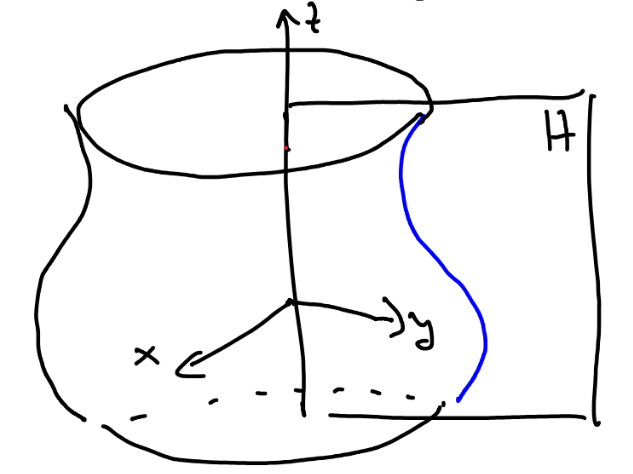
\includegraphics[width=6cm]{6_6 rot.png}
			\wrapincfig{6_6 rot}{6cm}
		\end{wrapfigure}
		Die von $\iota: S_C \hookrightarrow \R^3$ auf $S_C$ induzierte Metrik $\iota^*\bar{g}$ berechnet man lokal mit Parametrisierungen (wie oben):\\
		Sei $ \gamma(t) = (a(t),b(t)) $ eine lokale Parametrisierung von $C$. Dann ist
		\[ \varphi(t,\theta) = \big( a(t)\cos(\theta), a(t)\sin(\theta),b(t) \big) \]
		eine lokale Parametrisierung von $S_C$.
	\end{minipage}
	\begin{align*}
		\varphi^*\bar{g} &= d\big( a(t)\cos(\theta) \big)^2 + d\big( a(t)\sin(\theta) \big)^2 + d\big( b(t) \big)^2\\
		&= \big( \underbrace{a'(t)^2 + b'(t)^2}_{\|\gamma'(t)\|^2} \big)dt^2 + a(t)^2d\theta^2
	\end{align*}
\end{exmp*}

\subsection*{}

\begin{defn*}[(lokale) Isometrie]
	Sei $ f:M \to N $ glatt und $ (M,g_M),(N,g_N) $ Riemannsche Mannigfaltigkeiten. $f$ heißt \emph{Isometrie}, falls $f$ ein Diffeomorphismus ist und 
	$$f^*g_N = g_M.$$
	$f$ heißt \emph{lokale Isometrie}, falls $f$ ein lokaler Diffeomorphismus ist, der $ f^*g_N = g_M $ erfüllt.
\end{defn*}

\begin{rem}
	lokaler Diffeomorphismus: $ \foralll p \in M \ \existss U \subset M $ offen, $p \in U$, sodass $ \bound{f}{p} $ ein Diffeomorphismus auf $f(U)$ (offen in $N$) ist. Beachten Sie: $f$ ist genau dann ein lokaler Diffeomorphismus, wenn $ df_p: T_pM \to T_{f(p)}N $ ein Isomorphismus ist. (Das zeigt man in Koordinaten mit Hilfe des Satzes von der Umkehrfunktion auf Diff 2)
\end{rem}

\begin{exmp*}
	für einen lokalen, nicht globalen Diffeomorphismus
	\begin{itemize}
		\item $t \mapsto e^t, \R \to \R,$ ist nicht surjektiv.
		\item $ f: \R^2 \to \R^2, f(x,y) = (e^x\cos(y),e^x\sin(y)) $ ist nicht injektiv ($2\pi$-Periodizität)
	\end{itemize}
\end{exmp*}

\begin{defn*}
	Eine Metrik heißt \emph{flach}, falls sie lokal isometrisch zur euklidischen Metrik ist.
\end{defn*}

\begin{thm}\label{6.8}
	Sei $ (M,g) $ eine Riemannsche Mannigfaltigkeit. Dann sind äquivalent:
	\begin{enumerate}[label={\roman*})]
		\item $g$ ist flach
		\item $ \foralll p \in M \ \existss U \subset M $ offen, $p \in U, \varphi: U \to \R^n$ Karte, sodass in lokalen Koordinaten bezüglich $\varphi$ gilt:
			\[ g = \sum \delta_{ij} dx^i dx^j \]
	\end{enumerate}
\end{thm}

\begin{rem*}
	ACHTUNG: In Bemerkung \ref{6.1} hatten wir für ein fest gewähltes $p \in M$ eine Basis von $ T_pM $ gewählt, die $g_p$ in die Form $ \begin{pmatrix}
		1&&\\&\ddots&\\&&1
	\end{pmatrix} $ bringt. Die Aussage von \ref{6.8} ist stärker! Hier gibt es eine \emph{offene} Menge $ U \subset M $, auf der $g$ diese Form annimmt!
\end{rem*}

\begin{rem}
	$g$ flach $ \iff \foralll p \in M \ \existss U \subset M $ offen, $p \in U$ und ein kommutierendes orthonormales Vielbein\\
	kommutierend: $ \bound{(X_j \circ X_i - X_i \circ X_j)}{p} = 0 \qquad \foralll p \in U $
\end{rem}

\begin{lem}
	Sei $C$ eine zusammenhängende 1-dimensionale Untermannigfaltigkeit, eingebettet in $ H = \{r,z \mid r<0\} $. Sei $S_C$ die zugehörige Rotationsfläche. Dann ist $ \iota^*\bar{g} $ genau dann flach, wenn $C$ ein (offenes) Streckenstück ist.
\end{lem}

\subsection*{Riemannsche Mannigfaltigkeit $\to$ metrischer Raum:}

Für Kurven $ \gamma: I \to \R^n $ kennen wir schon die Länge 
\[ \int_I \|\gamma'(t)\|_E dt. \]
Analog betrachten wir nun zu einem stückweise glatten $ \gamma: [a,b] \to M $ ($(M,g)$ Riemannsche Mannigfaltigkeit)
\[ L_g(\gamma) = \int_a^b \|\gamma'(t)\|_g dt \quad \text{"Länge von $\gamma$"} \]
\[ \|\gamma'(t)\|_g = \sqrt{g_{\gamma(t)} (\gamma'(t), \gamma'(t))} \]

\begin{rem}
	\begin{enumerate}[label={\roman*})]
		\item $\gamma'$ ist außerhalb einer endlichen Menge von Punkten $\in [a,b]$ definiert und dort auch stetig und in anderen Punkten sind rechts- und linksseitige Grenzwerte definiert $\implies$ Integral ist wohldefiniert.
		\item Wie im Fall von Kurven im $\R^n$ zeigt man für ein stückweise glattes $\gamma: [a,b] \to M$:
		\[ L_g(\gamma) = L_g (\bound{\gamma}{[a,c]}) + L_g (\bound{\gamma}{[c,b]}) \]
		für $a \leq c \leq b$ und $L_g(\gamma)$ ist von der Parametrisierung unabhängig.
	\end{enumerate}
\end{rem}

\begin{lem}\label{6.12}
	Sei $ f: M \to N $ auf Riemannschen Mannigfaltigkeiten $(M,g_M)$ und $(N,g_N)$ eine lokale Isometrie. Dann ist $ L_{g_N}(f \circ \gamma) = L_{g_M} (\gamma) $ für die stückweise glatte Kurve $\gamma: [a,b] \to M$.
\end{lem}

\begin{defn*}[Riemannscher Abstand]\index{Riemannscher Abstand}
	Sei $ (M,g) $ eine zusammenhängende Riemannsche Mannigfaltigkeit und $ p,q \in M $. Dann nennt man
	\[ d_g(p,q) = \inf \{L_g(\gamma) \mid \gamma\ \text{stückweise glatte Kurve von $p$ nach $q$} \} \]
	den \emph{Riemannschen Abstand} von $p$ zu $q$.
\end{defn*}

\begin{rem*}
	Wir haben im Lemma gesehen, dass immer eine stückweise glatte Kurve existiert ($M$ zusammenhängend).
\end{rem*}

\begin{rem*}
	In $ (\R^n,\bar{g}) $ gilt: $ d_g(p,q) = \|p-q\|_E $ (kürzeste Verbindung: Streckenstück)
\end{rem*}
\lecture\begin{rem}
	Wegen \ref{6.12} ist die Definition von $d_g$ unabhängig von der Koordinatenwahl in $M$.
\end{rem}

\begin{rem}
	Direkt aus der Definition sieht man:
	\begin{itemize}
		\item $ d(p,p) = 0, d(p,q) \geq 0 $
		\item $ d(p,q) = d(q,p) $ ($L(\gamma)$ ist unabhängig von der Umlaufrichtung)
		\item $ d(p,q) \leq d(p,\tilde{q}) + d(\tilde{q},q) $
	\end{itemize}
\end{rem}

\begin{thm}
	$ (M,d_g) $ ist ein metrischer Raum.
\end{thm}

\begin{lem}
	Sei $ p \in M,$ $(M,g) $ eine Riemannsche Mannigfaltigkeit. Dann ist $ f:= d_g(\cdot,p) $ stetig.
\end{lem}

\begin{cor}
	Die Topologie auf $ (M,g) $, die von $d_g$ induziert wird, ist die selbe wie die Topologie auf $M$ als Mannigfaltigkeit.
\end{cor}

\begin{lem}
	Sind $ (M,g_M), (N,g_N) $ zusammenhängende Riemannsche Mannigfaltigkeiten, $ f:M \to N $ eine Isometrie, so gilt
	\[ d_{g_N}(f(p),f(q)) = d_{g_M}(p,q) \quad \foralll p,q \in M. \]
\end{lem}

\begin{rem*}
	Lokale Isometrien können in der Tat Länge verkürzen.\\
	\begin{minipage}{\linewidth}
		\begin{wrapfigure}{r}{4cm}
			%			\centering
			\wrapincfig{6_18 rem}{4cm}
		\end{wrapfigure}
		$ f: \R \to \R^2$\\
		$f(t) = (\cos(t),\sin(t)) $ ($ \im(f) = \Sbb^1 $)\\
		$ d_{\Sbb^1}(p,q) = $ Bogenlänge = $ |t-t_0| \mod 2\pi $\\
		$ d_\R(t,t_0) = |t-t_0| \geq |t-t_0| \mod 2\pi $
	\end{minipage}
\end{rem*}

\begin{cor*}
	Eine zusammenhängende Riemannsche Mannigfaltigkeit $M$ ist genau dann \emph{vollständig} (als topologischer Raum) wenn $(M,d_g)$ vollständig ist (als metrischer Raum).\\
	Und: Es ist sinnvoll, eine Teilmenge $ A \subset M $ beschränkt zu nennen, falls $ \existss C \geq 0 $, sodass $ d_g(q,p) \leq C \ \foralll q,p \in A. $
\end{cor*}

\begin{exmp*}
	nicht vollständig: $ \Sbb^2 \setminus \{p\} $\\
	$ d(q_1,q_2) = $ Bogenlänge der Verbindung auf dem (kürzeren) Großkreis
	\incfig{6_18 exmp}{3cm}
\end{exmp*}

\begin{rem*}
	"Geodäte" =  eine kürzeste Verbindung zwischen zwei Punkten.\\
	Muss nicht existieren (siehe oben)
\end{rem*}

\begin{rem}
	$ \hat{g}: TM \to T^*M, \hat{g}(v)(w) := g_p(v,w) \ \foralll v,w \in T_pM $\\
	$ Y \mapsto \hat{g}(X)(Y) $ ist $C^\infty$-linear, $X,Y \in \Xfrak(M)$\\
	\ref{4.7} $\implies \hat{g}(X)$ ist ein glattes Vektorfeld \checkmark \\
	$\hat{g}$ ist ein Isomorphismus:\\
	injektiv wegen $\hat{g}(v) = 0 \implies 0 = \langle v,v\rangle_g \implies 0$\\
	$\implies$ (Dimensionsformel) $\hat{g}$ surjektiv.
\end{rem}

\begin{defn*}[Gradient]
	Sei $f: M \to \R$ glatt auf $(M,g)$. Der \emph{Gradient} von $f$ ist
	\[ \grad f = \hat{g}^{-1}(df) \in \Xfrak(M) \]
\end{defn*}

\begin{rem*}
	\begin{enumerate}[label={\roman*})]
		\item Für $ M = \R^n, g = \bar{g}, $ ist $ \grad f = (\del{1}f \dots \del{n}f) $
		\item Es gilt $ \foralll X \in \Xfrak(M): $\\
			$ \langle \grad f, X \rangle_g = \hat{g} (\grad f)(X) = df(X) = X \cdot f $
		\item $\grad f$ zeigt in Richtung des stärksten Anstiegs und steht orthogonal auf den Höhenlinien.
	\end{enumerate}
\end{rem*}

\begin{exmp*}
	$\bar{g}$ in Polarkoordinaten: $ \begin{pmatrix}
		1&0\\0&r^2
	\end{pmatrix},\ \bar{g}^{-1} = \begin{pmatrix}
	1&0\\0&\frac{1}{r^2}
	\end{pmatrix} $\\
	$ \implies \grad f  = \del{r}f \cdot \del{r} + \frac{1}{r^2} \del{\theta}f \cdot \del{\theta} $
\end{exmp*}
	\chapter{Differentialformen}\lecture

Erinnerung an Kapitel \ref{4}:

\begin{defn*}[$k$-Form, $k$-Differentialform]\index{k@$k$-Form}\index{Differentialform}
	Ein Schnitt im Bündel der alternierenden (total anti-symmetrischen) kovarianten $k$-Tensoren über einer $n$-dimensionalen differenzierbaren Mannigfaltigkeit $M$,
	\[ \alpha: M \to \Lambda^k T^*M := \bigcup_{p \in M} \underbrace{\Lambda^k(T_p^*M)}_{\text{äußere Algebra}}, \]
	heißt \emph{$k$-Form}, ein glatter Schnitt heißt \emph{$k$-Differentialform} und $k$ heißt \emph{Grad}.
\end{defn*}

Den Vektorraum der $k$-Differentialformen bezeichnet man mit $\Omega^k(M)$. Das Dachprodukt wird punktweise definiert, also $ \bound{(\omega \wedge \eta)}{p} = \bound{\omega}{p} \wedge \bound{\eta}{p} $. Versehen mit $\wedge$ wird dann
	\[ \qquad \Omega^*(M) := \bigoplus_{k=0}^n \Omega^k(M) \qquad (\Omega^0(M) = C^\infty(M)) \]
zu einer Algebra.

\begin{rem*}
	In Koordinaten lässt sich $\omega \in \Omega^k(M)$ schreiben als
	\[ \omega = \sum_{i_1 < i_2 < \dots} \omega_{i_1\dots i_k} dx^{i_1} \wedge \dots \wedge dx^{i_k}. \]
\end{rem*}

\begin{lem}
	Es gilt
	\[ dx^{i_1} \wedge dx^{i_k} (\del{j_1}, \dotsc, \del{j_k}) = \delta_{j_1\dots j_k}^{i_1 \dots i_k} \]
	\[ \text{mit } \delta_{j_1\dots j_k}^{i_1 \dots i_k} = \det \begin{pmatrix}
		\delta_{j_1}^{i_1} & \dots & \delta_{j_k}^{i_1}\\
		\vdots & & \vdots\\
		\delta_{j_1}^{i_k} & \dots & \delta_{j_k}^{i_k}
	\end{pmatrix} \]
\end{lem}

\begin{cor*}
	$ \omega_{i_1 \dots i_k} = \omega(\del{i_1}, \dotsc, \del{i_k}) $
\end{cor*}

\begin{exmp*}
	\begin{itemize}
		\item[]
		\item $ \omega = \cos(x) dy \wedge dz + \sin(xy) dx \wedge dz \in \Omega^2(\R^3) $\\
			$ \omega_{23}(x,y,z) = \cos(x),\ \omega_{13}(x,y,z) = \sin(xy) $
			\begin{align*}
				\omega \wedge dy &= 0 +\sin(xy) dx \wedge dz \wedge dy\\
				&= -\sin(xy) dx \wedge dy \wedge dz\\
				\omega \wedge \omega &= 0
			\end{align*}
		
		\item $ \Omega^n(\R^n) = \big\{ f(x_1,\dotsc,x_n) dx^1 \wedge \dots \wedge dx^n \mid f \in C^\infty (\R^n) \big\} $
	\end{itemize}
\end{exmp*}

\begin{lem}
	Ist $ f: M \to N $ glatt, so gilt für den pullback einer Differentialform auf $N$ entlang $f$
	\[ \bound{f^*\omega}{p} (v_1,\dotsc,v_k) = \bound{\omega}{f(p)} (df_p(v_1),\dots, df_p(v_k)) \quad (p \in M, v_j \in T_pM) \]
	\begin{enumerate}[label={\roman*})]
		\item $ f^*: \Omega^k(N) \to \Omega^k(M) $ linear
		\item $ f^*(\omega \wedge \eta) = f^*\omega \wedge f^*\eta $
		\item $ f^*\left(\sum\limits_{i_1 < i_2<\dots} \omega_{i_1\dots i_k} dx^{i_1} \wedge \dots \wedge dx^{i_k}\right) = \sum\limits_{i_1<i_2<\dots} ( \omega_{i_1\dots i_k} \circ f) d(x^{i_1} \circ f) \wedge \dots \wedge d(x^{i_k} \circ f) ) $
	\end{enumerate}
\end{lem}

\begin{exmp*}
	$ f: \R^2 \to \R^3, f(u,v) = (u,v,u^2), \omega = y dy \wedge dz \in \Omega^2(\R^3) $
	\begin{align*}
		\bound{f^*\omega}{(u,v)} &= \big(\underbrace{y \circ f}_{=v}(u,v) \big) d(\underbrace{y \circ f}_{v} )|_{(u,v)} \wedge \underbrace{d(\underbrace{z \circ f}_{u^2})|_{(u,v)}}_{2udu}\\
		&= -2uv\, du \wedge dv
	\end{align*}
\end{exmp*}

\begin{exmp*}
	Kartenwechsel ($ f = \id $, aber im Urbild und Bild werden verschiedene Koordinaten verwendet)
	\begin{align*}
		\omega &= dx \wedge dy \qquad \begin{pmatrix}
			x\\y
		\end{pmatrix} = \begin{pmatrix}
		r\cos\theta\\r\sin\theta
	\end{pmatrix}\\
			&= d(r\cos\theta) \wedge d(r\sin\theta) \\
			&= (\cos\theta dr - r\sin \theta d \theta) \wedge (\sin\theta dr + r\cos\theta d \theta)\\
			&= rdr \wedge d\theta
	\end{align*}
\end{exmp*}

Das ist kein Zufall:

\begin{lem}
	Sei $ f: M \to N $ glatt, $ \dim M = \dim N = n $. Seien $ x_1,\dotsc,x_n $ Koordinaten bei $p \in M$ und $ y_1,\dotsc,y_n $ Koordinaten bei $ f(p) \in N $. Dann gilt für $ \omega \in \Omega^n(N),\ \omega = u dy^1 \wedge \dots \wedge dy^n $ ($u \in C^\infty(N)$):
	\[ f^*\omega = (u \circ f)(\det \vertarrowbox[1ex]{Df}{Jacobimatrix von $f$}) dx^1 \wedge \dots \wedge dx^n \]
	auf $ U \cap f^{-1}(V) $ ($U$ Koordinaten bei $p$, $V$ Koordinaten bei $f(p)$).
\end{lem}

\begin{cor*}
	Sind $ (x_1,\dotsc,x_n) $ und $ (y_1,\dotsc,y_n) $ Koordinaten, so gilt auf dem Überlappungsbereich
	\[ dy^1 \wedge \dots \wedge dy^n = \det \frac{\del{y_j}}{\del{x_i}} dx^1 \wedge dx^n \]
\end{cor*}

\begin{exmp*}
	$ \begin{pmatrix}
		x\\y
	\end{pmatrix} = \begin{pmatrix}
		r\cos\theta\\r\sin\theta
	\end{pmatrix} $
	\begin{align*}
		dy \wedge dy &= \det \begin{pmatrix}
			\del{r}(r\cos\theta) & \del{\theta}(r\cos\theta)\\
			\del{r}(r\sin\theta) & \del{\theta}(r\sin\theta)
		\end{pmatrix} dr \wedge d\theta\\
		&= r\big(\cos\theta^2 + \sin\theta^2\big) dr \wedge d\theta
	\end{align*}
\end{exmp*}

\begin{defn*}
	Sei $ \omega \in \Omega^k(M), X \in \Xfrak(M) $. Man definiert punktweise eine $(k-1)$-Form durch
	\[ \bound{(X \lrcorner \omega)}{p} := X_p \lrcorner \omega_p := \iota_{X_p} \omega_p, \]
	wobei $ \iota_v \alpha (v_1, \dotsc,v_{k-1}) := \alpha(v,v_1,\dotsc,v_{k-1}) $ für $v,v_j \in V, \alpha \in \Lambda^kV^*$ das \emph{innere Produkt von $\alpha$ mit $v$} bzw. \emph{$\omega$ mit $X$} oder die \emph{Einsetzung von $X$ in $\omega$} ist.
\end{defn*}

\begin{rem}
	\begin{enumerate}[label={\roman*})]
		\item $ \iota_X \omega \in \Omega^{k-1}(M), \omega \in \Omega^k $
		\item $ \iota_v \circ \iota_v = 0 $
		\item $ \iota_v(\omega \wedge \eta) = \iota_v(\omega) \wedge \eta + (-1)^k \omega \wedge (\iota_v \eta) $ wenn $ \omega \in \Omega^k(M) $
	\end{enumerate}
\end{rem}
Erinnerung: \lecture $ \omega \in \Omega^1(M) $ heißt geschlossen, falls $ \del{i}\omega_j . \del{j} \omega_i = 0 $ lokal in jeder Karte.\\
Idee: Definiere eine Abbildung $ d: \Omega^1 \to \Omega^2 $, die in Koordinaten gegeben ist als
\[ d\omega = d \big( \sum \omega_j dx^j \big) = \sum_{i < j} (\del{i} \omega_j - \del{j} \omega i) dx^i \wedge dx^j \]
Geschlossenheit wäre dann gleichbedeutend mit $d\omega = 0$.

\begin{defn}[äußere Ableitung, Cartan-Ableitung]\index{äußere Ableitung} \index{Cartan-Ableitung} \label{7.5}
	Sei $ V \subset \R^n $ offen. Sei $ \omega \in \Omega^k(V) $, also 
	\[ \omega = \sum_{i_1 < \dots < i_k} \omega_{i_1 \dots i_k} dx^{i_1} \wedge \dots \wedge dx^{i_k}. \]
	Dann definieren wir die \emph{äußere Ableitung} oder \emph{Cartan-Ableitung} $d\omega$ \emph{von $\omega$} vermöge
	\[ d\omega := \sum_{i_1 < \dots < i_k} \sum_j \del{j} \omega_{i_1 \dots i_k} dx^j \wedge dx^{i_1} \wedge \dots \wedge dx^{i_k}. \]
\end{defn}

\begin{rem*}
	\begin{enumerate}[label={\roman*})]
		\item $ \omega = f \in C^\infty(M) = \Omega^0(M) $\\
			$ df = \sum_j \del{j} f dx^j = df $ im Sinne der Definition
		\item $ \omega \in \Omega^1(M) $
			\begin{align*}
				d\omega &= \sum_j \sum_i \del{j}\omega_i dx^j \wedge dx^i = \sum_{j<i} \dotsc + \sum_{j > i} \dots\\
				&= \sum{j<i} (\del{j} \omega_i - \del{i}\omega_j) dx^j \wedge dx^i
			\end{align*}
	\end{enumerate}
\end{rem*}

\begin{lem}
	Es gilt für $ V,W \subset \R^n $ offen
	\begin{enumerate}[label={\roman*})]
		\item $ d: \Omega^k(V) \to \Omega^{k+1}(V) $ linear
		\item $ d(\omega \wedge \eta) = d\omega \wedge \eta + (-1)^k \omega \wedge d\eta $ für $ \omega \in \Omega^k(V), \eta \in \Omega^l(V). $
		\item $d \circ d = 0$
		\item $ f: V \to W $ glatt, $\omega \in \Omega^k(W): f^*(d\omega) = d(f^*\omega)$
	\end{enumerate}
\end{lem}

\begin{thm}
	Ist $M$ eine differenzierbare Mannigfaltigkeit, so gibt es eine eindeutige lineare Abbildung $ d: \Omega^k(M) \to \Omega^{k+1}(M) $, sodass
	\begin{gather*}
		d(\omega \wedge \eta) = d\omega \wedge \eta + (-1)^k \omega \wedge d \eta \qquad \foralll \omega \in \Omega^k, \eta \in \Omega^l\\
		d \circ d = 0.
	\end{gather*}
	Für $ f \in \Omega^0 = C^\infty $ gilt:
	\begin{gather*}
		df \ \text{ist das Differential von $f$, also}\\
		df(X) = X(f) \qquad \foralll X \in \Xfrak^1(M)
	\end{gather*}
	In lokalen Koordinaten ist $d\omega$ gegeben wie in \ref{7.5}.
\end{thm}

\addtocounter{thm}{-1}

\begin{lem}
	$ f: M \to N $ glatt mit differenzierbaren Mannigfaltigkeiten $M,N$. Dann gilt
	\[ f^*(d\omega) = d(f^*\omega) \qquad \foralll \omega \in \Omega^k(N). \]
\end{lem}
\lecture

Erinnerung: \begin{enumerate}[label={\roman*})]
	\item $ d: \Omega^k(M) \to \Omega^{k+1}(M) $ Cartan Ableitung (Satz \ref{7.7})
	\item Satz \ref{3.40} (Lemma von Poincaré):\\
		Auf sternförmigen Gebieten sind geschlossene Formen $\omega \in \Omega^1(M)$ exakt, das heißt $\existss \alpha$, sodass $\omega = d\alpha$.
	\item \label{erinnerung} $ \omega = \frac{1}{x^2+y^2}(xdy - ydx) $ ist auf
		\begin{itemize}
			\item $\R^2 \setminus \{0\}$ geschlossen, aber nicht exakt
			\item auf $\{(x,y) \mid x>0\}$ exakt (und immer noch geschlossen) (mit $\alpha = \arctan \frac{y}{x}$)
		\end{itemize}
\end{enumerate}

Das heißt wir erfahren etwas über den zugrunde liegenden Raum, wenn wir Formen auf Exaktheit/Geschlossenheit untersuchen.

\begin{defn}[geschlossene und exakte $k$-Formen]
	\begin{align*}
		\Zcal^k(M) &:= \ker \left( d: \Omega^k(M) \to \Omega^{k+1}(M) \right)\\
			&= \{ \text{"geschlossene $k$-Formen"} \}\\
		\Bcal^k(M) &:= \im \left( d: \Omega^{k-1}(M) \to \Omega^k(M) \right)\\
			&= \{ \text{"exakte $k$-Formen"} \}
	\end{align*}
\end{defn}

\begin{rem*}
	\begin{enumerate}[label={\roman*})]
		\item Für $k<0$ und $k>\dim M = n$: $ \Omega^k(M) = \{0\} $, also z.B. $ \Zcal^n(M) = \Omega^n(M) $ und $ \Bcal^0(M) = \{0\}. $
		\item Für $k=1$ stimmt die Definition von Geschlossenheit mit unserer bisherigen überein.
	\end{enumerate}
\end{rem*}

\begin{defn}[de-Rham-Kohomologie-Gruppe]\index{de-Rham-Kohomologie-Gruppe}
	Man nennt den Quotienten-Vektorraum
	\[ \drco{k}{M} = \frac{\Zcal^k(M)}{\Bcal^k(M)} \]
	die \emph{$k$-te de-Rham-Kohomologie-Gruppe}.
\end{defn}

\begin{rem*}
	\begin{itemize}
		\item Der Quotient kann gebildet werden, da wegen $d \circ d = 0$ gilt: $\Bcal^k(M) \subseteq \Zcal^k(M)$
		\item Sei $\omega \in \Zcal^k(M)$, dann ist $[\omega] \in \drco{k}{M}$:
			\[ [\omega] = \big\{ \eta \in \Zcal^k(M) \mid \omega - \eta \in \Bcal^k(M) \big\} \]
			Ist $[\omega] = [\tilde{\omega}]$, so nennt man $\omega$ \emph{kohomolog} zu $\tilde{\omega}$.
		\item Die Gruppenoperation ist die Addition.
		\item $ \drco{k}{M} = 0 $ für $k<0, k > \dim M$
		\item Für $ 0 \leq k \leq \dim M $ gilt $ \drco{k}{M} = 0 $ genau dann, wenn jede geschlossene $k$-Form exakt ist.
	\end{itemize}
\end{rem*}

\begin{exmp*}
	$ \drco{1}{U} = 0 $ für jedes sternförmige Gebiet $U \subseteq \R^n$\\
	$ \drco{1}{\R^2 \setminus \{0\}} \neq 0 $ (siehe \ref{erinnerung})
\end{exmp*}

\begin{lem}\label{7.14}
	Sind $M$ und $N$ zueinander diffeomorphe differenzierbare Mannigfaltigkeiten, so sind ihre Kohomologie-Gruppen isomorph, das heißt
	\[ \drco{k}{M} \cong \drco{k}{N}. \]
\end{lem}

\noindent Dies folgt direkt aus

\begin{lem}[Verhalten unter Pullback]
	Sei $ f: M \to N $ glatt. Dann gilt
	\begin{align*}
		f^*\big(\Zcal^k(N)\big) &\subset \Zcal^k(M) \quad \text{und}\\
		f^*\big(\Bcal^k(N)\big) &\subset \Bcal^k(M).
	\end{align*}
	Somit induziert $f^*$ auf $\drco{}{N}$ eine wohldefinierte Abbildung
	\begin{align*}
		f^*: \drco{k}{N} &\to \drco{k}{M}\\
		f^*[\omega] &:= [f^*\omega].
	\end{align*}
	Zudem gilt:
	\begin{enumerate}[label={\roman*})]
		\item Ist $g: N \to P$ eine weitere glatte Abbildung, so ist
			\[ (g \circ f)^* = f^* \circ g^*: \drco{k}{P} \to \drco{k}{M}. \]
		\item Ist $\id: M \to M$ die Identität, so ist $ \id^*: \drco{k}{M} \to \drco{k}{M} $ die Identität.
	\end{enumerate}
\end{lem}

Die Aussage aus \ref{7.14} folgt in der Tat sofort, weil in dem Fall $ f^*: \drco{k}{N} \to \drco{k}{M} $ ein Isomorphismus ist.

\begin{rem}\label{7.16}
	Tatsächlich gilt etwas viel Allgemeineres:\\
	Die de-Rham-Kohomologie ist von der differenzierbaren Struktur unabhängig, tatsächlich eine topologische Invariante, das heißt wenn es einen Homöomorphismus $M \to N$ (glatte Mannigfaltigkeiten) gibt, so gilt schon $ \drco{k}{M} \cong \drco{k}{N} $.
\end{rem}

\noindent Eine elementare Berechnung:

\begin{lem}\label{7.17}
	Betrachte $ M = \bigsqcup_{j \in J} M_j $ disjunkte Vereinigung, $J$ endlich, $M_j$ differenzierbare Mannigfaltigkeiten. Dann ist 
	\[ \drco{k}{M} \cong \bigoplus_{j \in J} \drco{p}{M_j}. \]
\end{lem}

\begin{cor*}
	Es genügt, zusammenhängende Mannigfaltigkeiten $M$ zu betrachten.
\end{cor*}

\begin{lem}
	$M$ zusammenhängend $\implies \drco{0}{M} = \{  f $ konstant$\}$ 
\end{lem}

\begin{cor}\label{7.19}
	Sei $ M = \{ p_1, \dotsc, p_k \} $ eine Mannigfaltigkeit der Dimension 0. Dann ist $ \drco{0}{M} = \bigoplus_{j=1}^k V_j $, wobei $V_j$ eindimensionale Vektorräume sind, und $\drco{k}{M} = 0$ für $k \geq 1$.
\end{cor}

\begin{rem*}
	\ref{7.17} und \ref{7.19} gelten auch im abzählbaren Fall.
\end{rem*}

Um \ref{7.16} zu verstehen müssen wir etwas weiter\footnote{Achtung! Folgende Ausführungen zu Homotopie sind \emph{Extrastoff} für besonders Interessierte und damit \emph{nicht klausurrelevant}. Allerdings sind sie als gute Übung im Rechnen mit $d$ und $\Omega^k$ zu betrachten.} ausholen:

\begin{defn}[Homotopie-Äquivalenz]\index{Homotopie-Äquivalenz}
	Eine stetige Abbildung $f: X \to Y$ zwischen topologischen Räumen heißt \emph{Homotopie-Äquivalenz}, falls es eine stetige Abbildung $g: Y \to X$ gibt, sodass $f \circ g$ homotop zu $\id_Y$ ist und $g \circ f$ homotop zu $\id_X$.\\
	Hierbei heißen zwei stetige Abbildungen $ \varphi_0, \varphi_1: X_1 \to X_2 $ \emph{homotop} zueinander, falls es eine stetige Abbildung $ H: X_1 \times [0,1] \to X_2 $ gibt mit
	\[ H(x,0) = \varphi_0(x),\quad H(x,1) = \varphi_1(x). \] Man schreibt dann $ \varphi_0 \cong \varphi_1 $. Tatsächlich ist Homotopie symmetrisch:
	\[ \tilde{H}(x,0) = \varphi_1(x), \quad \tilde{H}(x,1) = \varphi_0(x) \]
	für \( \tilde{H} = H \circ (\id \times \psi),\ \psi(t) = 1-t \).
\end{defn}

\begin{rem*}
	Man kann also die Abbildungen \( \varphi_0 \) und \( \varphi_1 \) (wenn sie homotop\footnote{$\underbrace{homo}_{"gleich"}\underbrace{top}_{"Ort"}$} zueinander sind) stetig ineinander Überführen (deformieren).
\end{rem*}

\begin{exmp*}%das mit dem Link
	
	\incfig{7_20a}{8cm}
	\( \Sbb^1 \times \Sbb^1 \) kann auch anders eingebettet werden, und zwar z.B. so:
	\incfig{7_20b}{12cm}
	Homotopie zwischen diesen Einbettungen:
	\href{https://en.wikipedia.org/wiki/Homotopy#/media/File:Mug_and_Torus_morph.gif}{GIF}
\end{exmp*}

\noindent Warum ist Homotopie-Äquivalenz hier wichtig?

\begin{thm}\label{7.21}
	Gibt es eine Homotopie-Äquivalenz zwischen zwei glatten Mannigfaltigkeiten $N$ und $M$, so gilt \( \drco{k}{M} \cong \drco{k}{N}. \)
\end{thm}

\begin{cor*}
	Sind $N$ und $M$ homöomorph, so gilt \( \drco{k}{M} \cong \drco{k}{N}. \)
\end{cor*}

Zum Beweis von \ref{7.21} benötigen wir einige Lemmata. Die Grundidee ist, dass zueinander homotope Abbildungen den selben Pullback auf der de-Rham-Kohomologie-Gruppe induzieren. Doch was heißt \( f^* = g^* \) auf \( \drco{k}{N} \)?

Seien $f,g: M \to N$ zwei glatte Abbildungen und $\omega \in \Zcal^k(N)$. Zu zeigen wäre, dass ein $\eta \in \Omega^{k-1}(M)$ existiert, sodass
\begin{equation}\label{eins}
	f^*\omega - g^*\omega = d\eta
\end{equation}
(denn dann würde \( f^*[\omega] - g^*[\omega] = [d\eta] = 0 \) gelten).\\
Ansatz: \( \eta = h_k(\omega) \) mit \( h_k: \Zcal^(N) \to \Omega^{k-1}(M) \)\\
Einfacher: Finde \( h_k: \Omega^(N) \to \Omega^{k-1}(M), k \in \N, \) sodass
\begin{equation}\label{zwei}
	d(h_k(\omega)) + h_{k+1}(d\omega) = f^*\omega - g^*\omega.
\end{equation}
Im Fall $d\omega = 0$ ist das Formel \ref{eins}.

\begin{notat*}
	Man schreibt wie beim Cartan-Differential nur $h$ und versteht darunter jeweils das zum jeweiligen Grad gehörige Element der Familie \( \{h_k\}_{k \in \N}. \)
\end{notat*}

\begin{defn*}[Homotopie-Operator] \index{Homotopie-Operator}
	Eine Familie linearer Abbildungen \( h: \Omega^k \to \Omega^{k-1} \) mit \ref{zwei} heißt \emph{(Ko-Ketten-) Homotopie-Operator} zwischen $f^*$ und $g^*$. 
\end{defn*}

\noindent Aus der Definition unmittelbar klar ist dann:

\begin{lem}
	Seien \( f,g: M \to N \) glatt und es gebe einen Homotopie-Operator zwischen $f^*$ und $g^*$. Dann sind die induzierten Abbildungen \( f^*,g^*: \drco{k}{N} \to \drco{k}{M} \) gleich.
\end{lem}

\subsection*{Existenz von Homotopie-Operatoren:}

\begin{lem}
	Sei \( \iota_0: M \to M \times [0,1], \iota_0(p) = (p,0) \) und \( \iota_1: M \to M \times [0,1], \iota_1(p) = (p,1). \) Dann gibt es einen Homotopie-Operator $h$ zwischen $\iota_0^*,\iota_1^*: \Omega^k(M \times [0,1]) \to  \Omega^k(M)$.
\end{lem}

\begin{prop*}
	\( h(d\omega) + d h(\omega) = \iota_1^*(\omega) - \iota_0^*(\omega) \)
\end{prop*}

\begin{lem}\label{7.24}
	Seien \( f,g: M \to N \) glatt und homotop zueinander mit einer \emph{glatten} Homotopie-Funktion \( H: M \times [0,1] \to N \) mit \( H(\cdot,0) = f, H(\cdot,1)=g \). Dann gilt 
	\[ f^*=g^*: \drco{k}{N} \to \drco{k}{M}. \]
\end{lem}

\begin{thm}[Whitney]
	Ist $f: M \to N$ stetig, so ist $f$ homotop zu einer glatten Abbildung.
	\incfig{7_25}{10cm}
\end{thm}

\begin{cor*}
	Sind \( f,g: M \to N \) glatt und homotop zueinander, so sind sie glatt homotop zueinander, also homotop mit einer glatten Homotopie-Funktion.
\end{cor*}

Insbesondere konnten wir also in \ref{7.24} o.B.d.A. annehmen, dass die Homotopie glatt ist. Damit folgen Satz \ref{7.21} und die Folgerung daraus.

Man kann diesen abstrakten Zugang anwenden, um \( \drco{k}{M} \) zu berechnen:

\begin{lem}
	Ist $M$ zusammensetzbar, ist also $\id_M$ homotop zu einer konstanten Abbildung, so ist \( \drco{k}{M} = 0 \ \foralll k \geq 1 \).
\end{lem}

\begin{thm}[Poincaré-Lemma]
	Ist $U \subseteq \R^n$ sternförmig, so ist \( \drco{k}{U} = 0 \ \foralll k \geq 1. \)
\end{thm}

\begin{cor*}
	Jeder Punkt $p \in M$ besitzt eine Umgebung auf der jede geschlossene Form ($k \geq 1$) exakt ist.
\end{cor*}
	
	
	
	
	
	

	\printindex
\end{document}